\documentclass{beamer}
\usepackage[utf8]{inputenc}
\usepackage{graphicx, epsfig}
\usepackage{amsmath,mathrsfs,amsfonts,amssymb}
%\usepackage{subfig}
\usepackage{floatflt}
\usepackage{epic,ecltree}
\usepackage{mathtext}
\usepackage{fancybox}
\usepackage{fancyhdr}
\usepackage{multirow}
\usepackage{enumerate}
\usepackage{epstopdf}
\usepackage{multicol}
\usepackage{algorithm}
\usepackage[noend]{algorithmic}
\def\algorithmicrequire{\textbf{Input:}}
\def\algorithmicensure{\textbf{Output:}}
\usetheme{default}%{Singapore}%{Warsaw}%{Warsaw}%{Darmstadt}
\usecolortheme{default}
\setbeamertemplate{footline}[page number]{}
\setbeamerfont{title}{size=\Huge}

\newcommand{\bc}{\mathbf{c}} 
\newcommand{\bt}{\mathbf{t}} 
\newcommand{\bu}{\mathbf{u}} 
\newcommand{\bv}{\mathbf{v}} 
\newcommand{\bw}{\mathbf{w}} 
\newcommand{\bx}{\mathbf{x}} 
\newcommand{\bz}{\mathbf{z}} 
\newcommand{\by}{\mathbf{y}} 

\newcommand{\bA}{\mathbf{A}} 
\newcommand{\bI}{\mathbf{I}} 
\newcommand{\bT}{\mathbf{T}} 
\newcommand{\bX}{\mathbf{X}} 
\newcommand{\bZ}{\mathbf{Z}} 

\newcommand{\bepsilon}{\boldsymbol{\epsilon}}
\newcommand{\bmu}{\boldsymbol{\mu}}
\newcommand{\blambda}{\boldsymbol{\lambda}}
\newcommand{\bsigma}{\boldsymbol{\sigma}}
\newcommand{\bSigma}{\boldsymbol{\Sigma}}

\newcommand{\bbE}{\mathbb{E}} 
\newcommand{\bbP}{\mathbb{P}} 
\newcommand{\bbR}{\mathbb{R}} 

\newcommand{\cL}{\mathcal{L}} 
\newcommand{\cN}{\mathcal{N}} 
\newcommand{\cS}{\mathcal{S}} 
\newcommand{\cX}{\mathcal{X}} 

\newcommand{\btheta}{\boldsymbol{\theta}} 
\newcommand{\bphi}{\boldsymbol{\phi}} 

\DeclareMathOperator*{\argmin}{arg\,min}
\DeclareMathOperator*{\argmax}{arg\,max}

%\definecolor{beamer@blendedblue}{RGB}{15,120,80}
%----------------------------------------------------------------------------------------------------------
\title[\hbox to 56mm{Deep Generative Models  \hfill\insertframenumber\,/\,\inserttotalframenumber}]
{Deep Generative Models \\ Lecture 11}
\author[Roman Isachenko]{\\Roman Isachenko}
\institute[MIPT]{Moscow Institute of Physics and Technology \\
}
\date{2020}
%--------------------------------------------------------------------------------
\begin{document}
%--------------------------------------------------------------------------------
\begin{frame}
%\thispagestyle{empty}
\titlepage
\end{frame}
%=======
\begin{frame}{Disentangled representations}
\begin{block}{Unsupervised representation learning}
    Learning an interpretable factorised representation of the independent data generative factors of the world without supervision. 
\end{block}
\begin{block}{Disentanglement informal definition}
A disentangled representation can be defined as one where single latent units are sensitive to changes in single generative factors, while being relatively invariant to changes in other factors. 
\end{block}
\begin{block}{Example}
Model trained on a dataset of 3D objects might learn independent latent units sensitive to single independent data generative factors, such as object identity, position, scale, lighting or colour. 
\end{block}
\vfill
\hrule\medskip
{\scriptsize \href{https://openreview.net/references/pdf?id=Sy2fzU9gl}{https://openreview.net/references/pdf?id=Sy2fzU9gl}}
\end{frame}
%=======
\begin{frame}{$\beta$-VAE, 2017}
\begin{block}{Generative process}
\begin{itemize}
    \item $p(\bx | \bv, \bw) = \text{Sim}(\bv, \bw)$~-- true world simulator;
    \item $\bv$~-- conditionally independent factors: $p(\bv | \bx) = \prod_{j=1}^d p(v_j | \bx)$;
    \item $\bw$~-- conditionally dependent factors. 
\end{itemize}
\end{block}
\begin{block}{Goal}
Construct an unsupervised deep generative model
\[
    p(\bx | \bz) \approx p(\bx | \bv, \bw).
\]
\vspace{-0.5cm}
\begin{itemize}
    \item Ensure that the inferred latent factors $q(\bz|\bx)$ capture the factors $\bv$ in a disentangled manner. 
    \item The conditionally dependent factors $\bw$ can remain entangled in a separate subset of $\bz$ that is not used for representing $\bv$. 
\end{itemize}
\end{block}
\vfill
\hrule\medskip
{\scriptsize \href{https://openreview.net/references/pdf?id=Sy2fzU9gl}{https://openreview.net/references/pdf?id=Sy2fzU9gl}}
\end{frame}
%=======
\begin{frame}{InfoGAN}
	\begin{block}{GAN objective}
		\vspace{-0.3cm}
		\[
		\min_{G} \max_D V(G, D)
		\]
		\[
		V(G, D)  =  \bbE_{\pi(\bx)} \log D(\bx) + \bbE_{p(\bz)} \log (1 - D(G(\bz)))
		\]
	\end{block}
	Latent vector $\bz$ is not imposed to be disentangled.
	
	InfoGAN decomposes input vector:
	\begin{itemize}
		\item $\bz$ -- incompressible noise;
		\item $\bc$ -- structured latent code $p(\bc) = \prod_{j=1}^d p(c_j)$.
	\end{itemize}
	\begin{block}{Information-theoretic regularization}
		\vspace{-0.3cm}
		\[
			\max I (\bc, G(\bz, \bc))
		\]
	\end{block}
	Information in the latent code $\bc$ should not be lost in the generation process.
	\vfill
	\hrule\medskip
	{\scriptsize \href{https://arxiv.org/abs/1606.03657}{https://arxiv.org/abs/1606.03657}}
\end{frame}
%=======
\begin{frame}{InfoGAN}
	\begin{block}{Objective}
		\vspace{-0.3cm}
		\[
		\min_{G} \max_D V(G, D) - \lambda I (\bc, G(\bz, \bc))
		\]
	\end{block}
	\begin{block}{Variational Information Maximization}
		\vspace{-0.3cm}
		\begin{multline*}
		I (\bc, G(\bz, \bc)) = H(\bc) - H(\bc | G(\bz, \bc)) = \\
		= H(\bc) + \bbE_{\bx \sim G(\bz, \bc)} \left[ \bbE_{\bc' \sim p(\bc | \bx)} \log p(\bc' | \bx) \right] = \\ 
		= H(\bc) + \bbE_{\bx \sim G(\bz, \bc)} KL(p(\bc'| \bx) || q(\bz' | \bx)) + 
		\\ + \bbE_{\bx \sim G(\bz, \bc)}  \bbE_{\bc' \sim p(\bc | \bx)} \log q(\bc' | \bx)  \geq\\
		 \geq H(\bc) + \bbE_{\bx \sim G(\bz, \bc)} \bbE_{\bc' \sim p(\bc | \bx)} \log q(\bc' | \bx) = \\
		 H(\bc) + \bbE_{\bc \sim p(\bc)} \bbE_{\bx \sim G(\bz, \bc)} \log q(\bc | \bx)
		\end{multline*}
	\end{block}
	\vfill
	\hrule\medskip
	{\scriptsize \href{https://arxiv.org/abs/1606.03657}{https://arxiv.org/abs/1606.03657}}
\end{frame}
%=======
\begin{frame}{InfoGAN}
	\begin{block}{Latent codes on MNIST}
		\begin{figure}
			\centering
			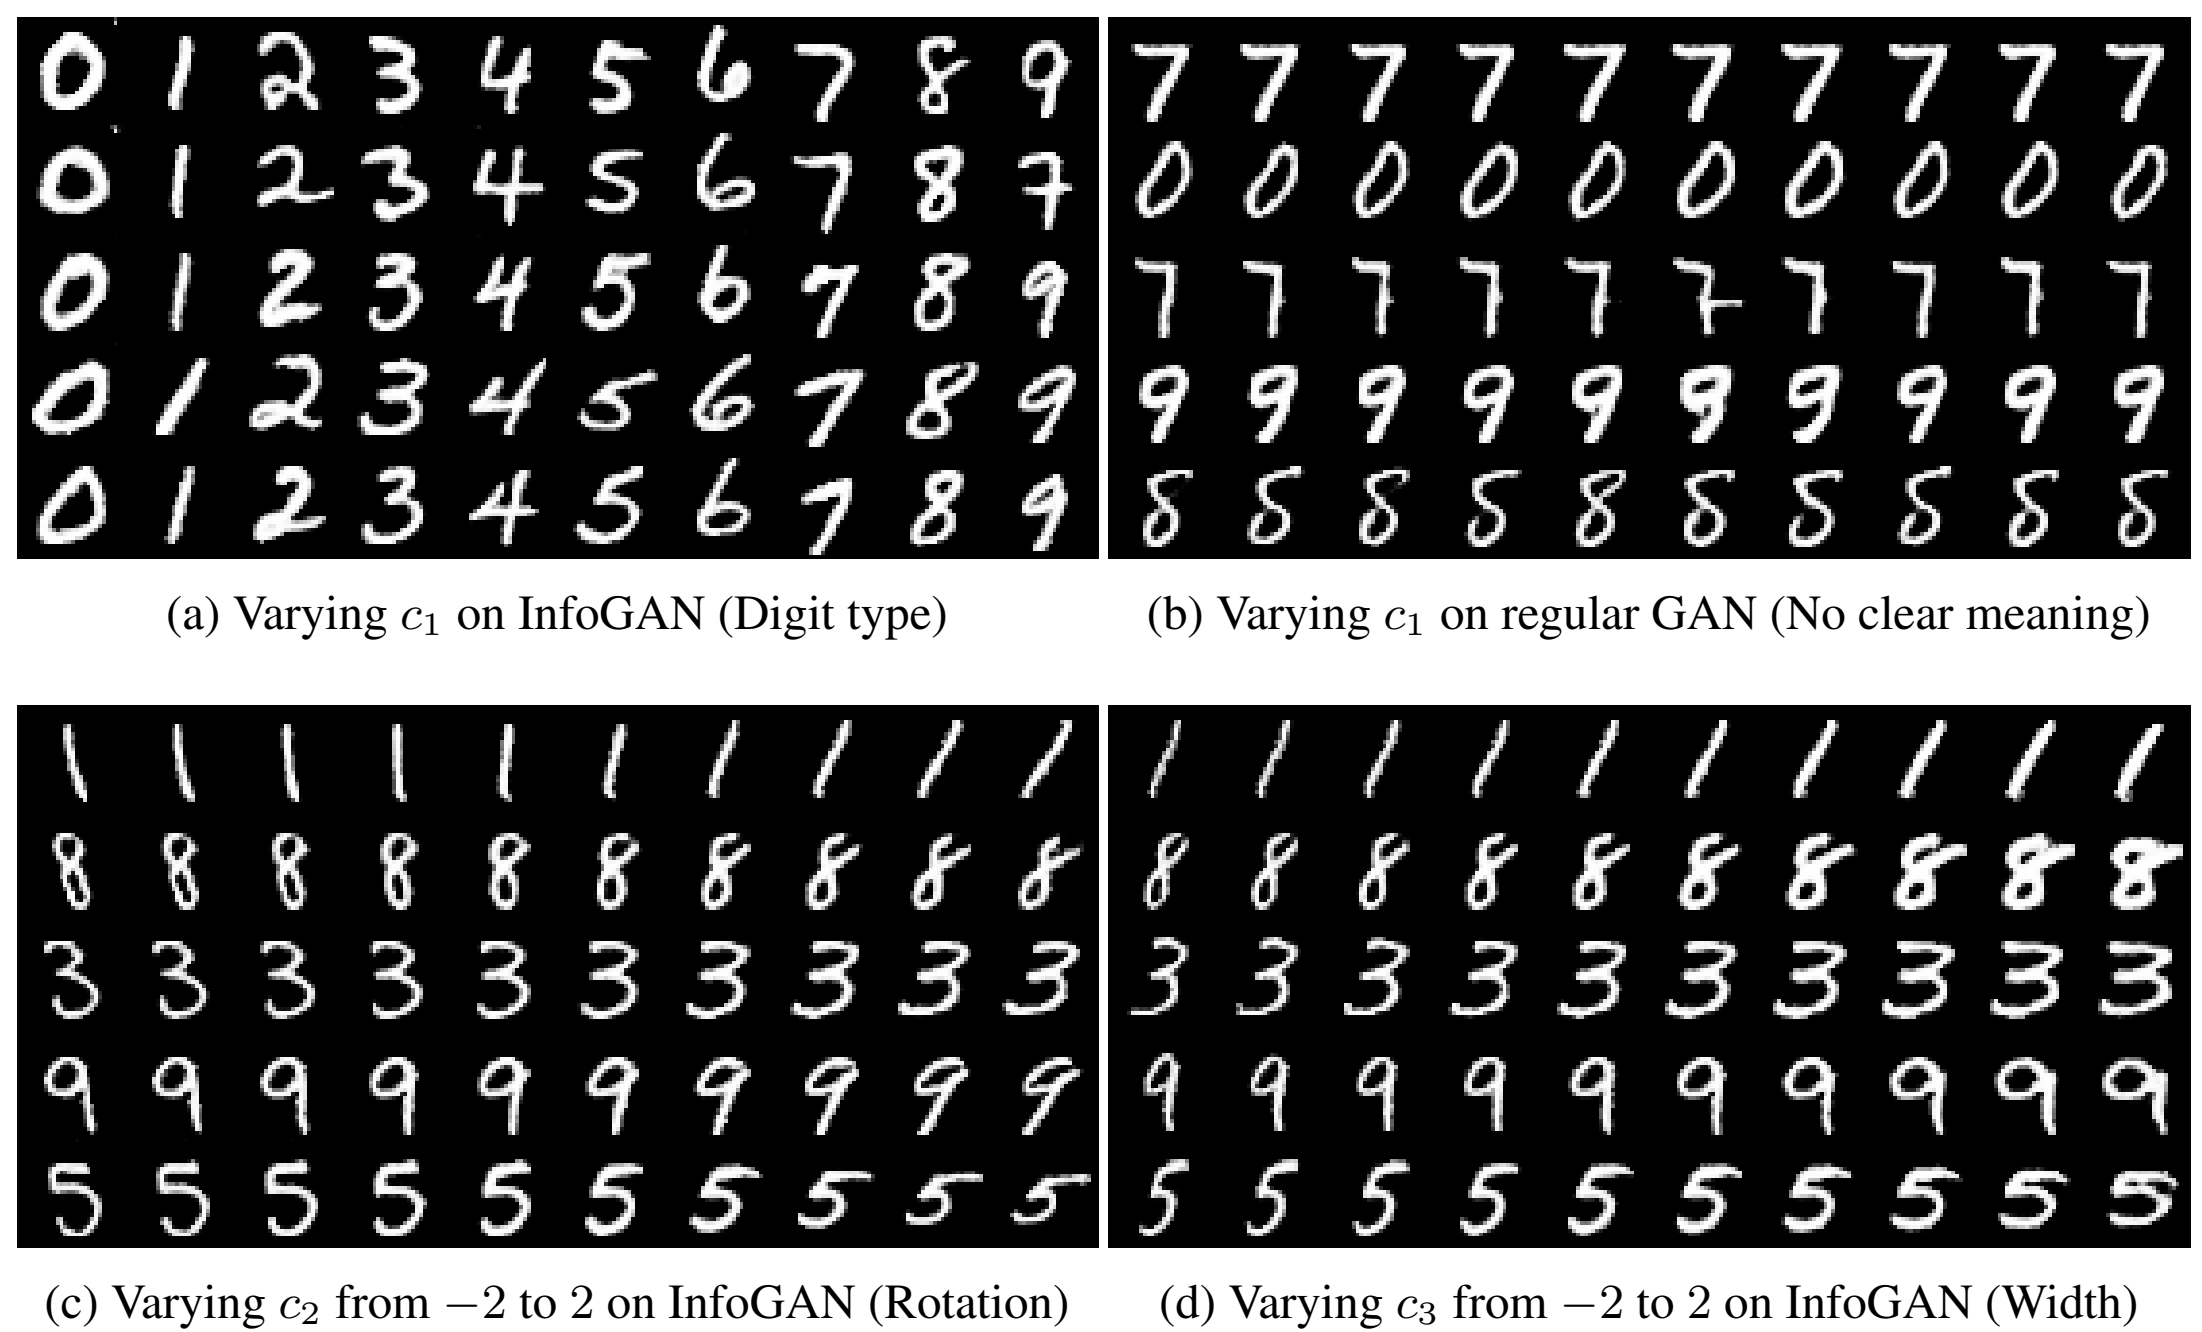
\includegraphics[width=\linewidth]{figs/infogan_mnist.png}
		\end{figure}
	\end{block}
	\vfill
	\hrule\medskip
	{\scriptsize \href{https://arxiv.org/abs/1606.03657}{https://arxiv.org/abs/1606.03657}}
\end{frame}
%=======
\begin{frame}{InfoGAN}
	\begin{block}{Latent codes on 3D Faces}
		\begin{figure}
			\centering
			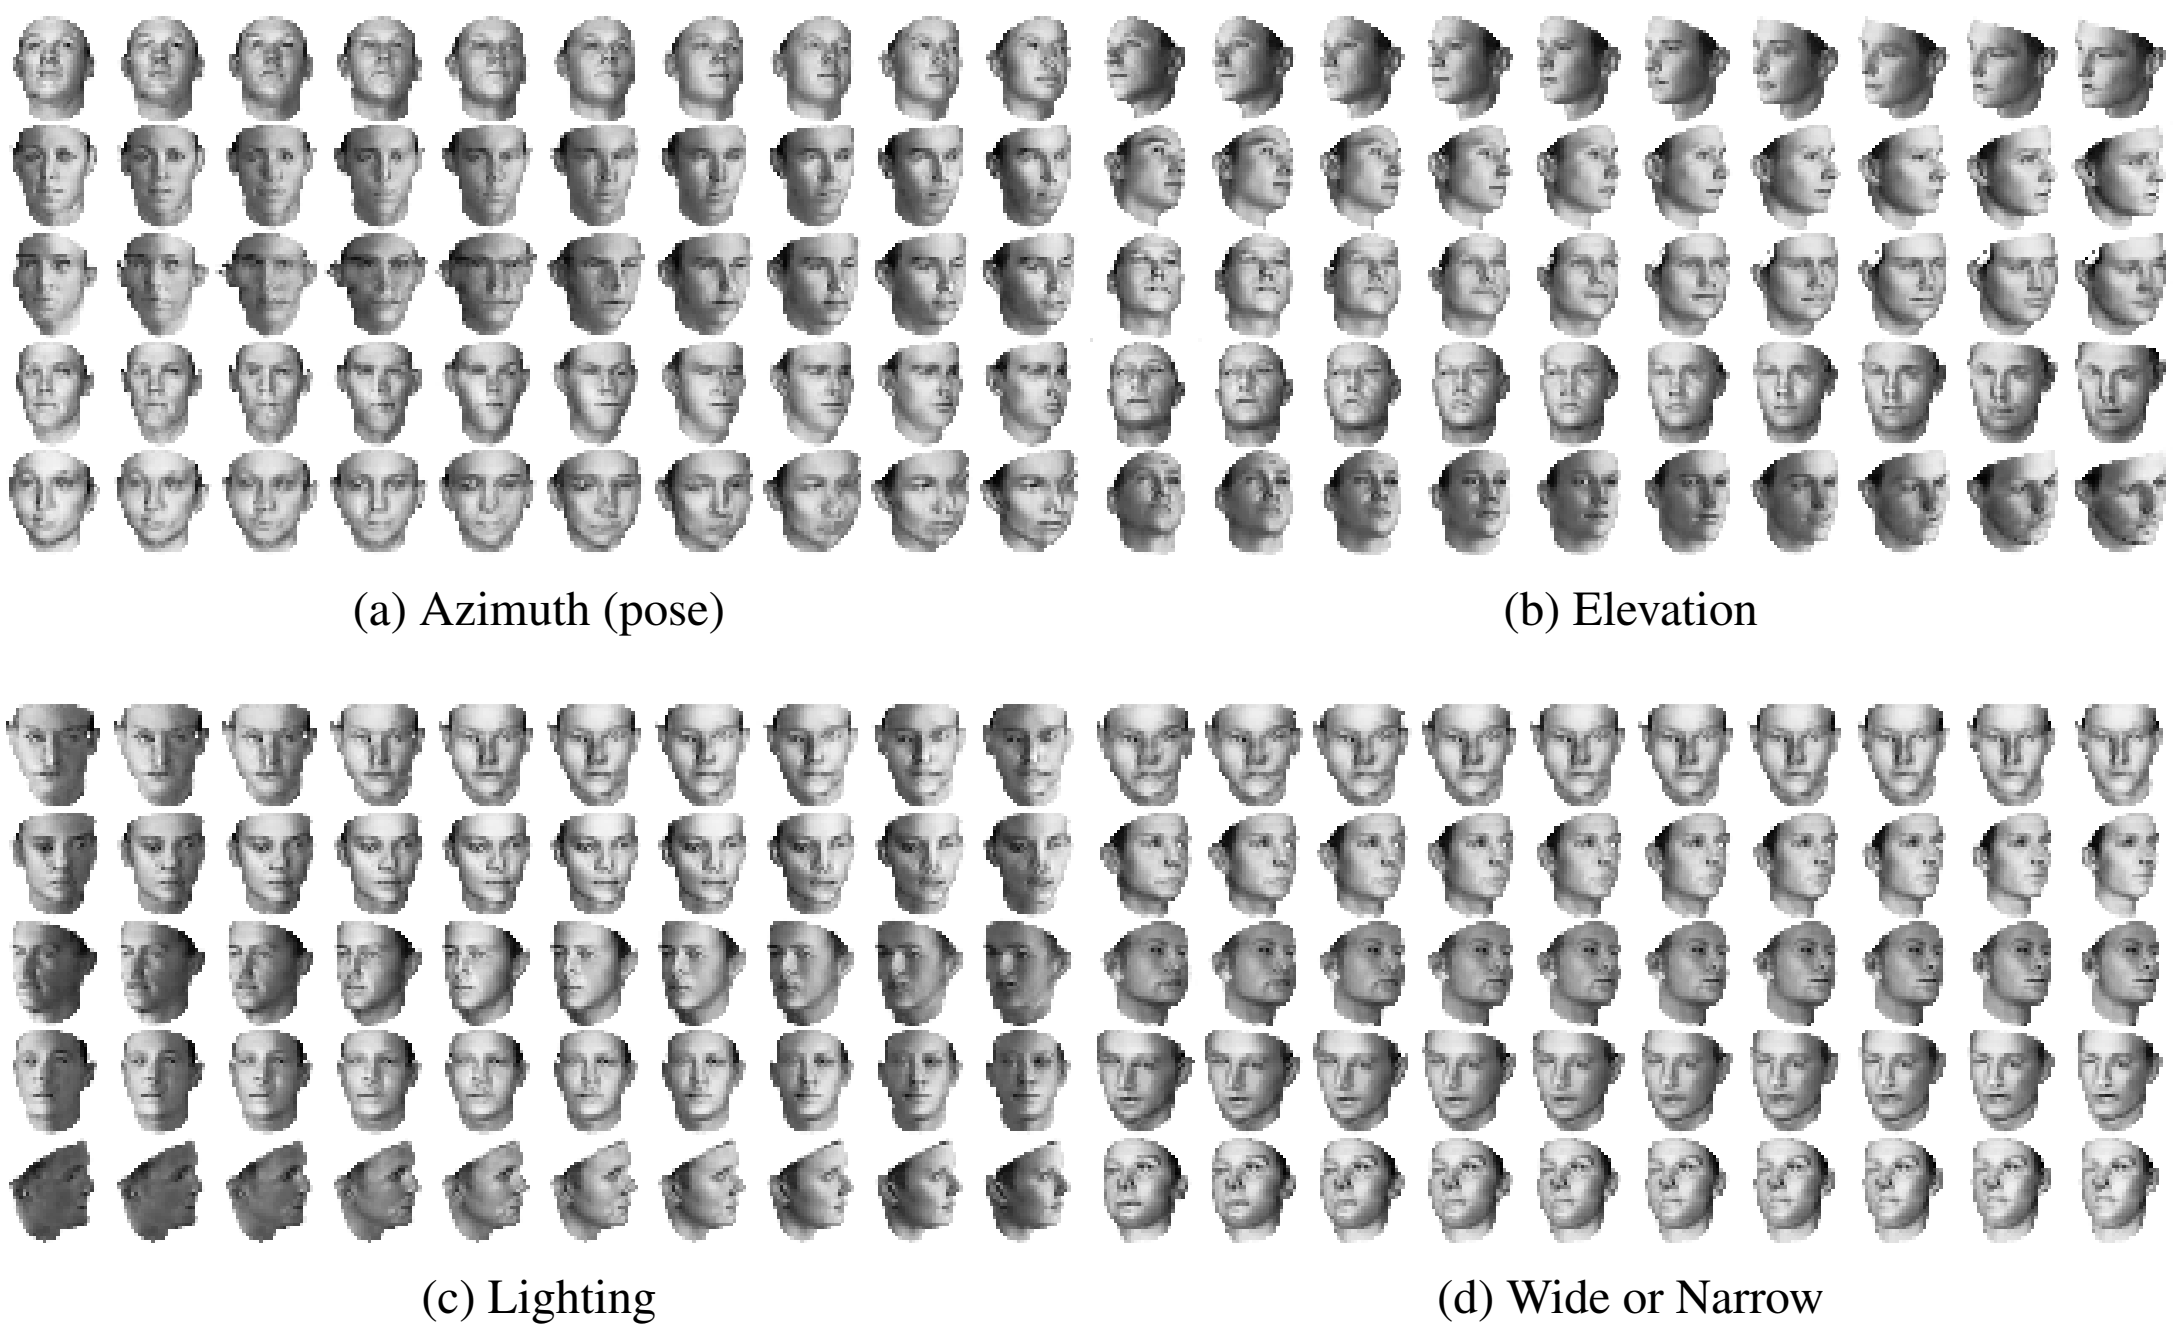
\includegraphics[width=\linewidth]{figs/infogan_faces.png}
		\end{figure}
	\end{block}
\vfill
\hrule\medskip
{\scriptsize \href{https://arxiv.org/abs/1606.03657}{https://arxiv.org/abs/1606.03657}}
\end{frame}
%=======
\begin{frame}{$\beta$-VAE}
\begin{block}{Constrained optimization}
\vspace{-0.5cm}
\[
    \max_{q, \btheta} \mathbb{E}_{q(\bz | \bx)} \log p(\bx | \bz, \btheta), \quad \text{subject to } KL (q(\bz | \bx) || p(\bz)) < \epsilon.
\]
\vspace{-0.5cm}
\end{block}
\begin{block}{Objective}
\vspace{-0.5cm}
\[
    \mathcal{L}(q, \btheta, \beta) = \mathbb{E}_{q(\bz | \bx)} \log p(\bx | \bz, \btheta) - \beta \cdot KL (q(\bz | \bx) || p(\bz)).
\]
\end{block}
What do we get at $\beta = 1$? \\
\begin{block}{Hypothesis}
To learn disentangled representations of the conditionally independent factors $\bv$, it is important to set stronger constraint on the latent bottleneck: $\beta > 1$.
\end{block}
\textbf{Note:} It could lead to poorer reconstructions due to the loss of high frequency details when passing through a constrained latent bottleneck. \\ 
\vspace{0.1cm}
\vfill
\hrule\medskip
{\scriptsize \href{https://openreview.net/references/pdf?id=Sy2fzU9gl}{https://openreview.net/references/pdf?id=Sy2fzU9gl}}
\end{frame}
%=======
\begin{frame}{$\beta$-VAE}
\begin{block}{Disentangling metric}
	\begin{enumerate}
		\item Generate two sets of objects
		\[
		\bx_{li} \sim \text{Sim}(\bv_{li}, \bw_{li}); \quad \bx_{lj} \sim \text{Sim}(\bv_{lj}, \bw_{lj}); \quad y_{ij} \sim U[1, d].
		\]
		\[
		\bv_{li} \sim p(\bv); \quad \bv_{lj} \sim p(\bv) \, ([v_{li}]_y = [v_{lj}]_y); \quad \bw_{li}, \bw_{lj} \sim p(\bw).
		\]
		\item Find representations
		\[
		q(\bz | \bx) = \mathcal{N}\left(\mu(\bx) | \sigma^2(\bx)\right); \quad \bz_{li} = \mu(\bx_{li}); \quad \bz_{lj} = \mu(\bx_{lj}).
		\]
		\item Use accuracy of classifier $p(y | \bz_{\text{diff}})$ with a low VC-dimension as metric of disentanglement
		\[
		\bz_{\text{diff}} = \frac{1}{L} \sum_{l=1}^L | \bz_{li} - \bz_{lj} |.
		\]
	\end{enumerate}

\end{block}

\vfill
\hrule\medskip
{\scriptsize \href{https://openreview.net/references/pdf?id=Sy2fzU9gl}{https://openreview.net/references/pdf?id=Sy2fzU9gl}}
\end{frame}
%=======
\begin{frame}{$\beta$-VAE}
\begin{figure}
    \centering
    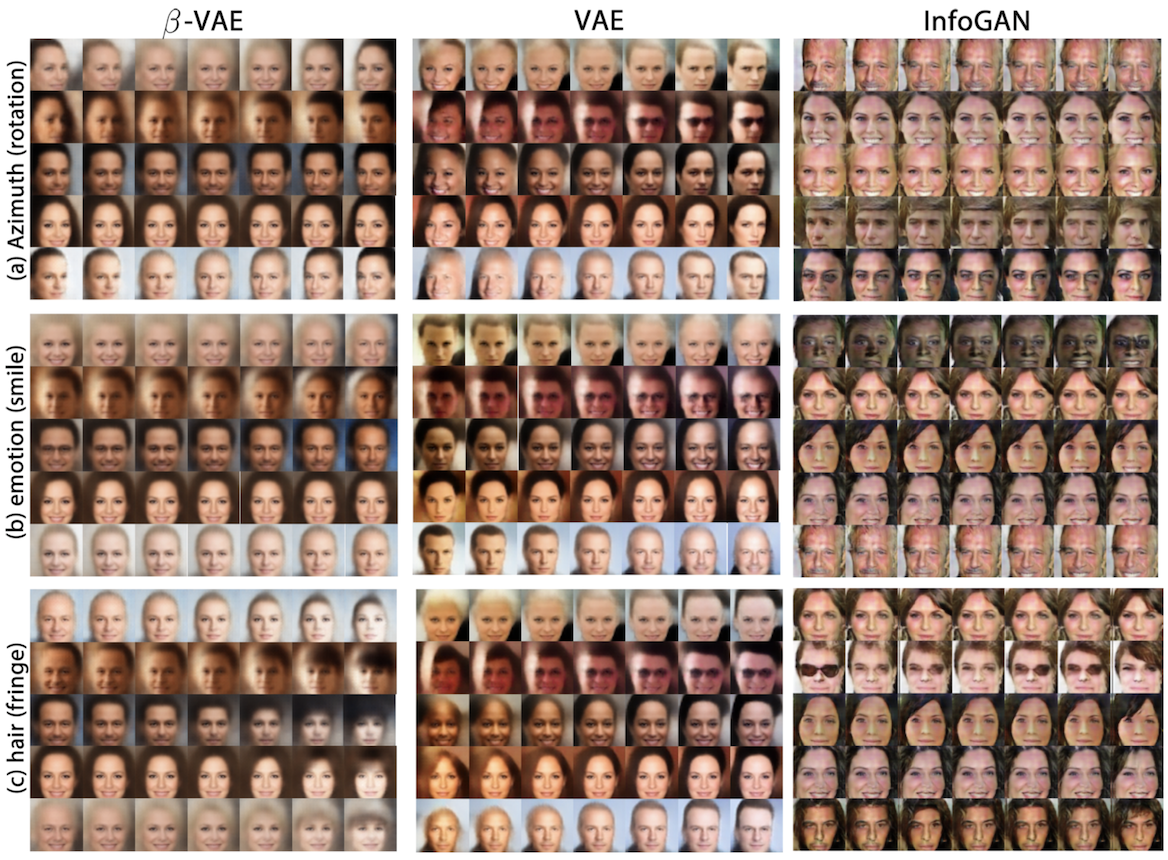
\includegraphics[width=0.95\linewidth]{figs/betaVAE_1.png}
\end{figure}
\vfill
\hrule\medskip
{\scriptsize \href{https://openreview.net/references/pdf?id=Sy2fzU9gl}{https://openreview.net/references/pdf?id=Sy2fzU9gl}}
\end{frame}
%=======
\begin{frame}{$\beta$-VAE}
\vspace{1cm}
\begin{figure}
    \centering
    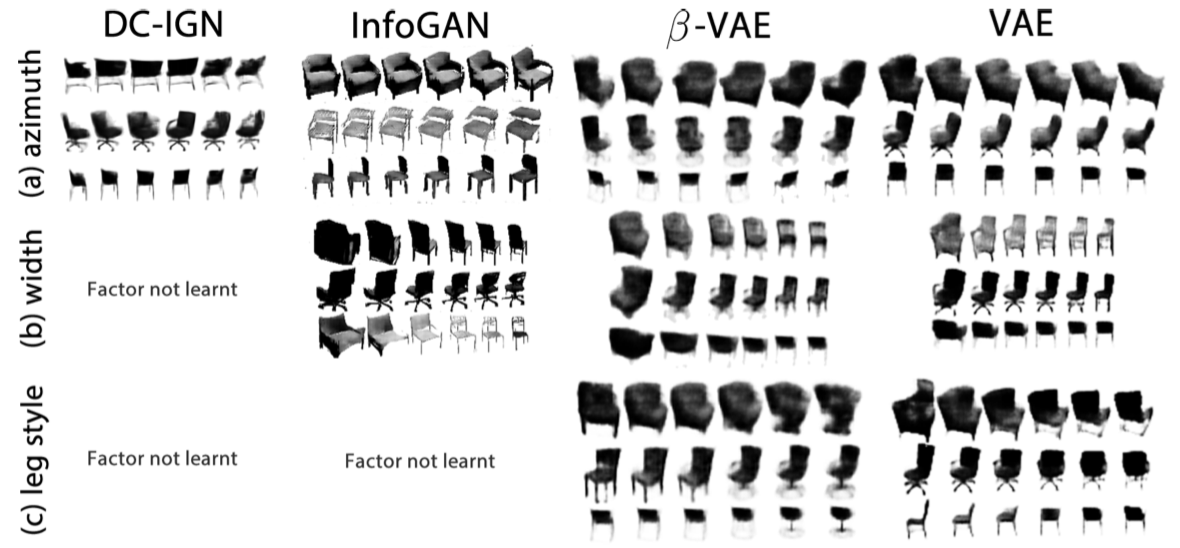
\includegraphics[width=\linewidth]{figs/betaVAE_2.png}
\end{figure}
\vspace{1cm}
\vfill
\hrule\medskip
{\scriptsize \href{https://openreview.net/references/pdf?id=Sy2fzU9gl}{https://openreview.net/references/pdf?id=Sy2fzU9gl}}
\end{frame}
%=======
\begin{frame}{$\beta$-VAE}
\begin{figure}
    \centering
    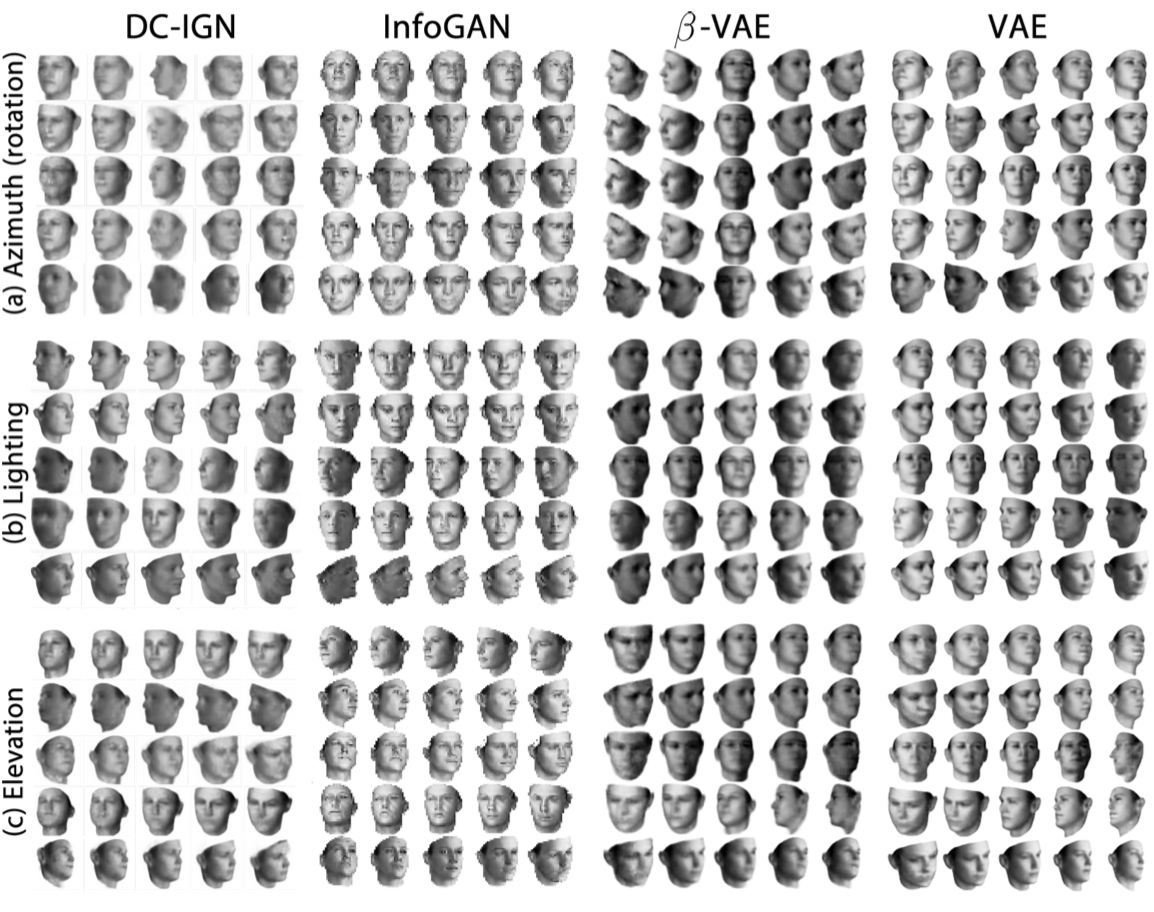
\includegraphics[width=0.8\linewidth]{figs/betaVAE_3.png}
\end{figure}
\vfill
\hrule\medskip
{\scriptsize \href{https://openreview.net/references/pdf?id=Sy2fzU9gl}{https://openreview.net/references/pdf?id=Sy2fzU9gl}}
\end{frame}
%=======
\begin{frame}{$\beta$-VAE}
	\begin{minipage}[t]{0.5\columnwidth}
	    \vspace{1.5cm}
		\begin{figure}
			\centering
			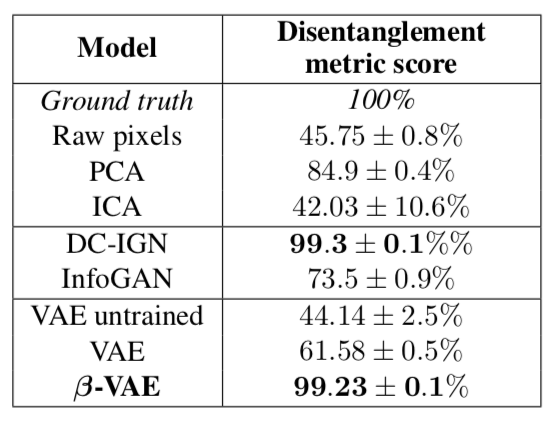
\includegraphics[width=1.\linewidth]{figs/betaVAE_4.png}
		\end{figure}
	\end{minipage}%
	\begin{minipage}[t]{0.5\columnwidth}
		\begin{figure}[h]
			\centering
			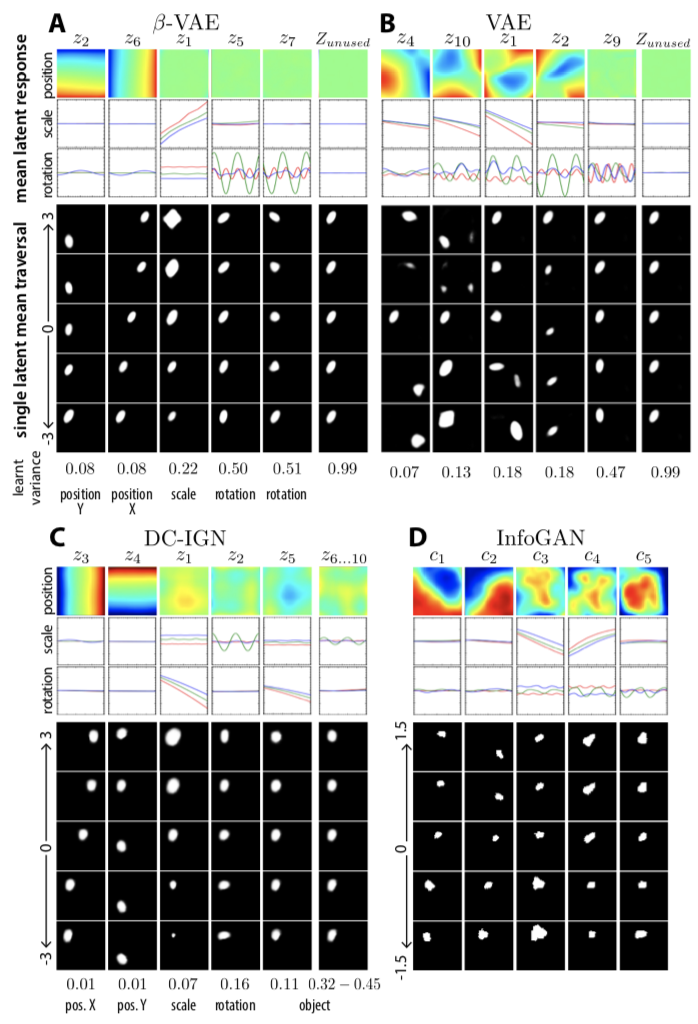
\includegraphics[width=.95\linewidth]{figs/betaVAE_5.png}
		\end{figure}
	\end{minipage}
\vfill
\hrule\medskip
{\scriptsize \href{https://openreview.net/references/pdf?id=Sy2fzU9gl}{https://openreview.net/references/pdf?id=Sy2fzU9gl}}
\end{frame}
%=======
\begin{frame}{$\beta$-VAE}
	\begin{itemize}
		\item \textbf{Top row:} original images.
		\item \textbf{Second row:} the corresponding reconstructions. 
		\item \textbf{Remaining rows:} latent traversals ordered by KL divergence with the prior. 
		\item \textbf{Heatmaps:} latent activations for each 2D position.
	\end{itemize}
\begin{figure}
    \centering
    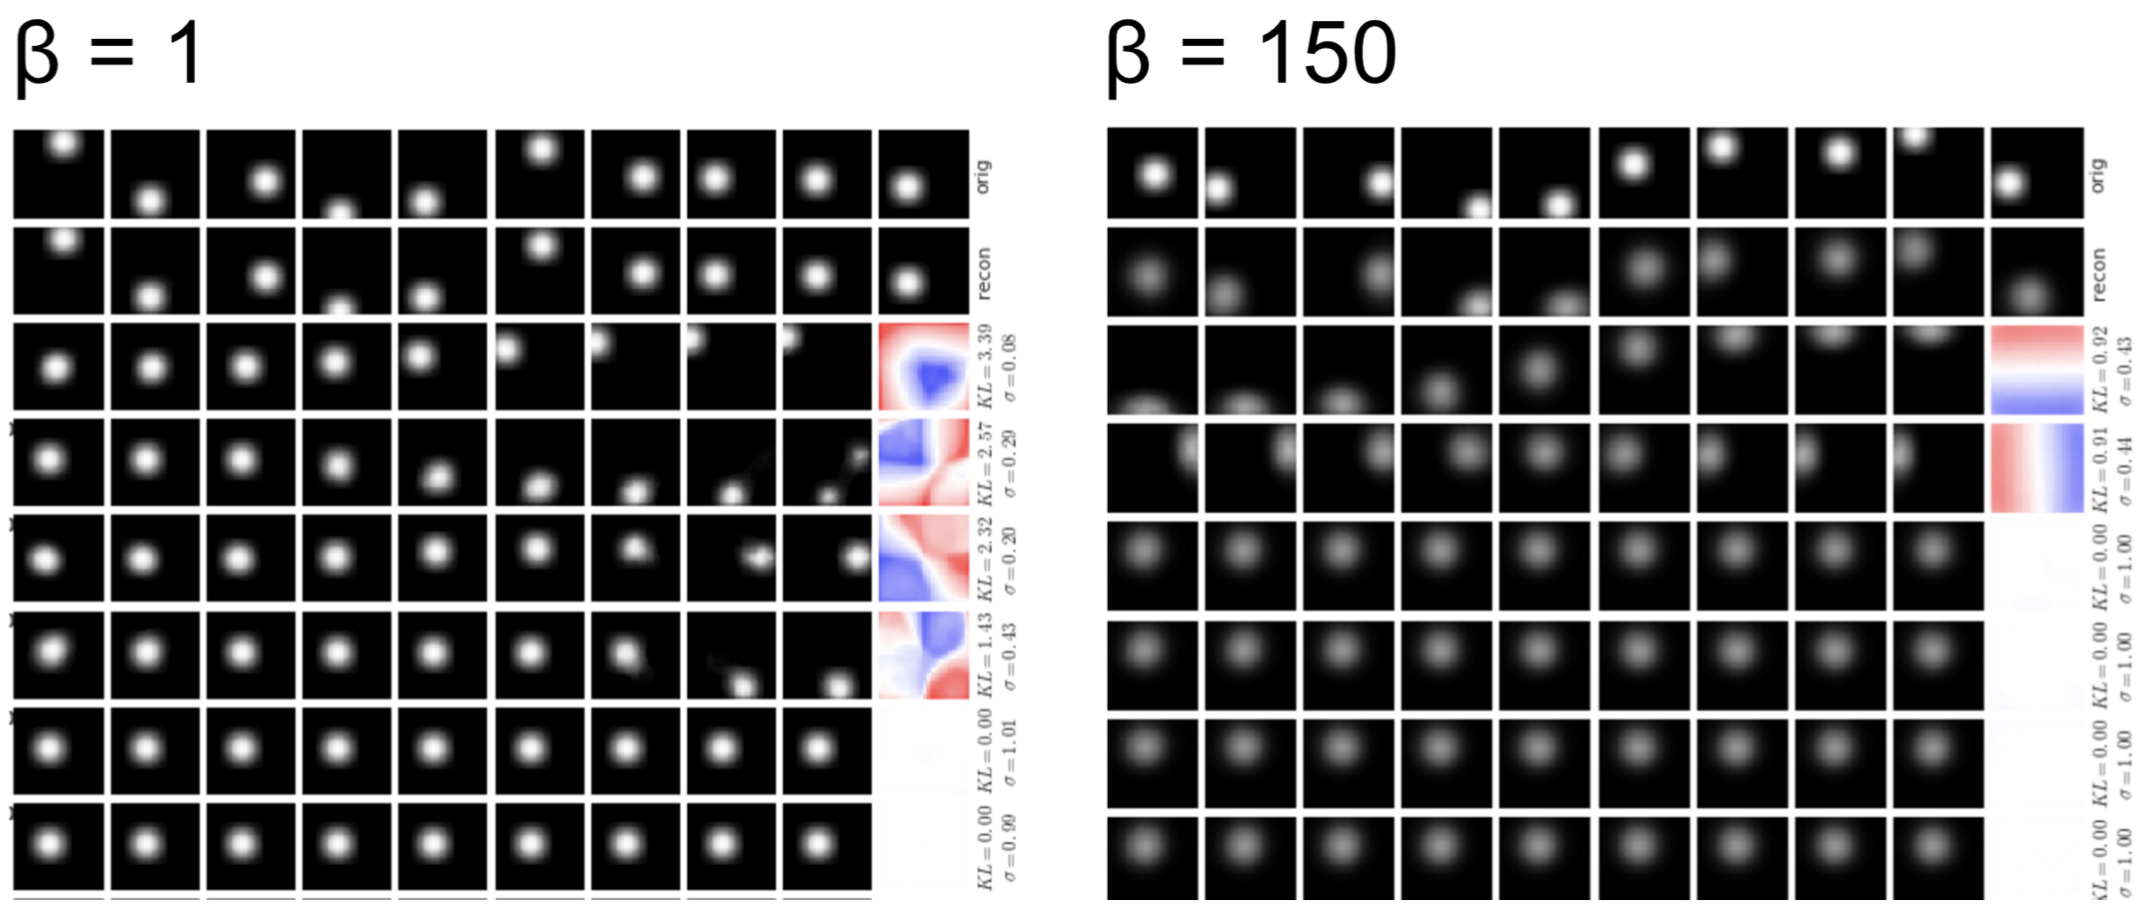
\includegraphics[width=\linewidth]{figs/betaVAE_6.png}
\end{figure}
\vspace{0.3cm}

\vfill
\hrule\medskip
{\scriptsize \href{https://arxiv.org/pdf/1804.03599.pdf}{https://arxiv.org/pdf/1804.03599.pdf}}
\end{frame}
%=======
\begin{frame}{$\beta$-VAE}
\begin{block}{Controlled encoding capacity}
\vspace{-0.5cm}
\[
    \mathcal{L}(q, \btheta, \beta) = \mathbb{E}_{q(\bz | \bx)} \log p(\bx | \bz, \btheta) - | KL (q(\bz | \bx) || p(\bz)) - C|.
\]
\end{block}
\begin{figure}
    \centering
    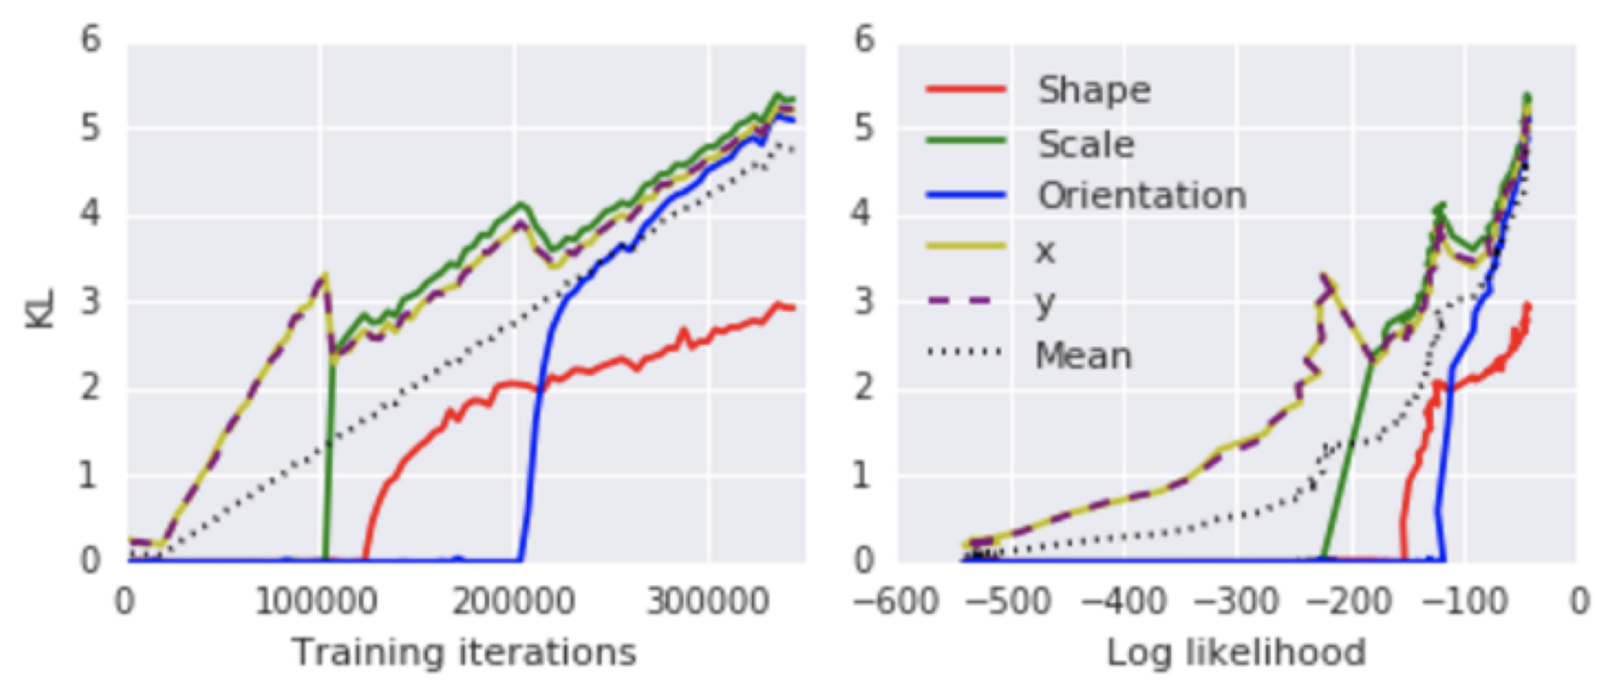
\includegraphics[width=0.9\linewidth]{figs/betaVAE_7.png}
\end{figure}
The early capacity is allocated to positional latents only, followed by a scale latent, then shape and orientation latents.
\vspace{0.3cm}

\vfill
\hrule\medskip
{\scriptsize \href{https://arxiv.org/pdf/1804.03599.pdf}{https://arxiv.org/pdf/1804.03599.pdf}}
\end{frame}
%=======
\begin{frame}{$\beta$-VAE}
\begin{block}{Controlled encoding capacity}
\vspace{-0.5cm}
\[
    \mathcal{L}(q, \btheta, \beta) = \mathbb{E}_{q(\bz | \bx)} \log p(\bx | \bz, \btheta) - | KL (q(\bz | \bx) || p(\bz)) - C|.
\]
\vspace{-0.5cm}
\end{block}
\begin{figure}
    \centering
    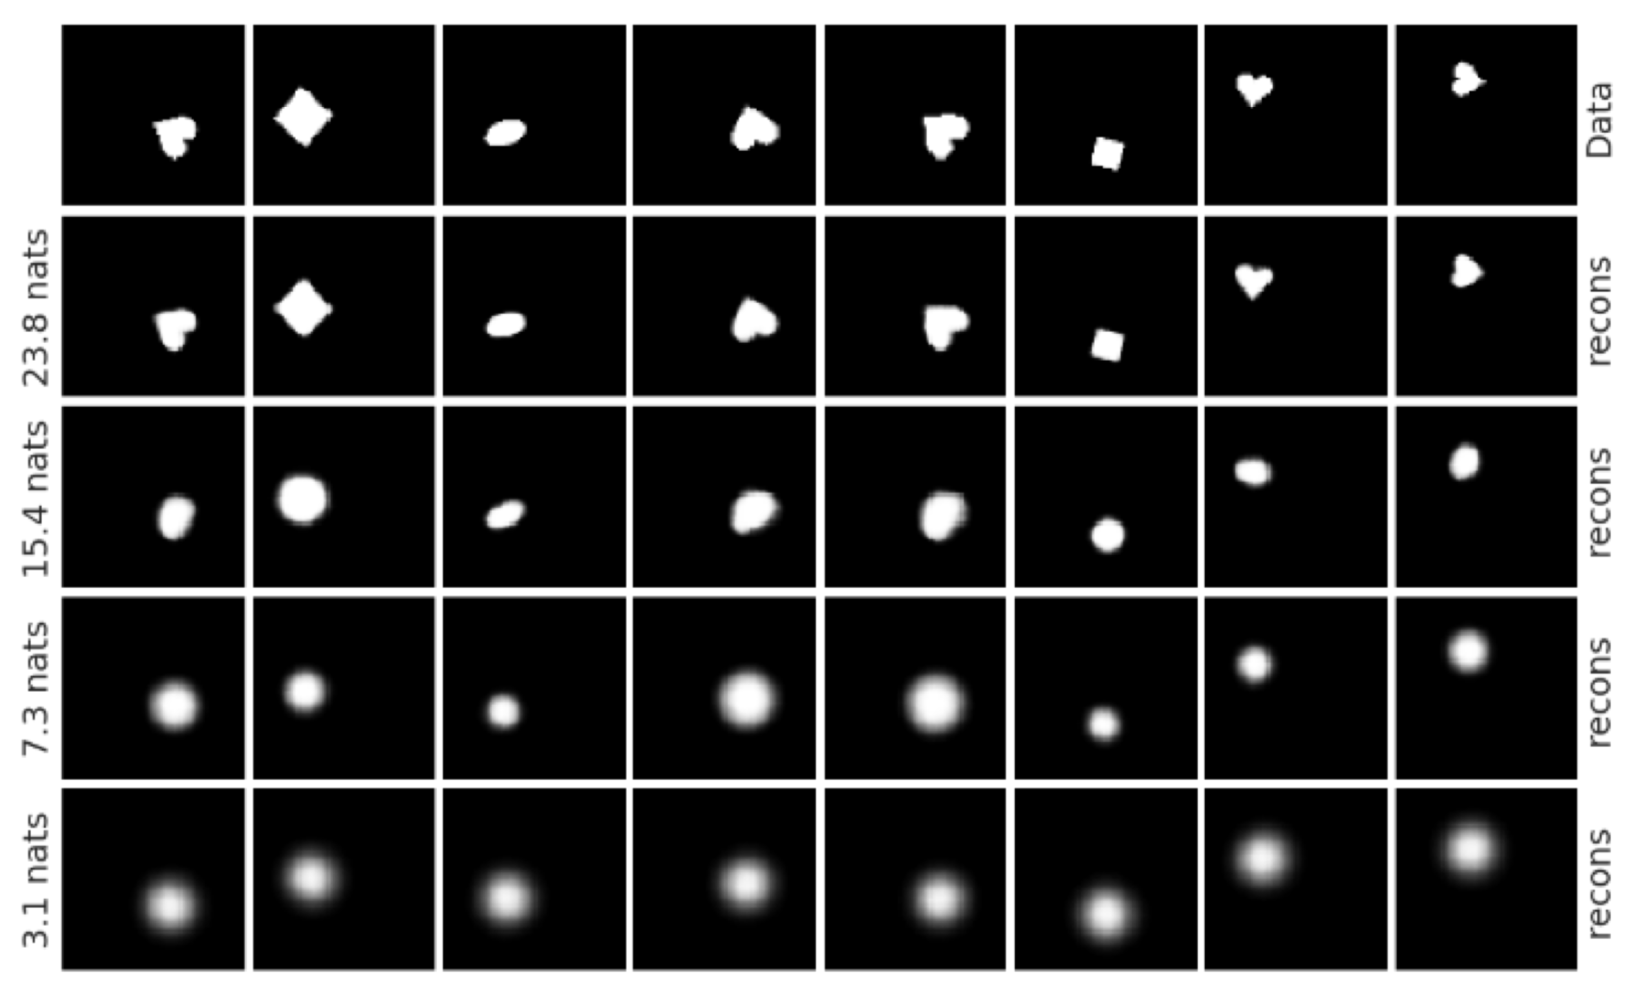
\includegraphics[width=0.7\linewidth]{figs/betaVAE_8.png}
\end{figure}
As the information capacity increases the different latents associated with their data generative factors become informative.
\vspace{0.3cm}

\vfill
\hrule\medskip
{\scriptsize \href{https://arxiv.org/pdf/1804.03599.pdf}{https://arxiv.org/pdf/1804.03599.pdf}}
\end{frame}
%=======
\begin{frame}{$\beta$-VAE}
	\begin{block}{Single latent traversals, ordered by their average KL divergence with the prior}
		\begin{figure}
		\centering
		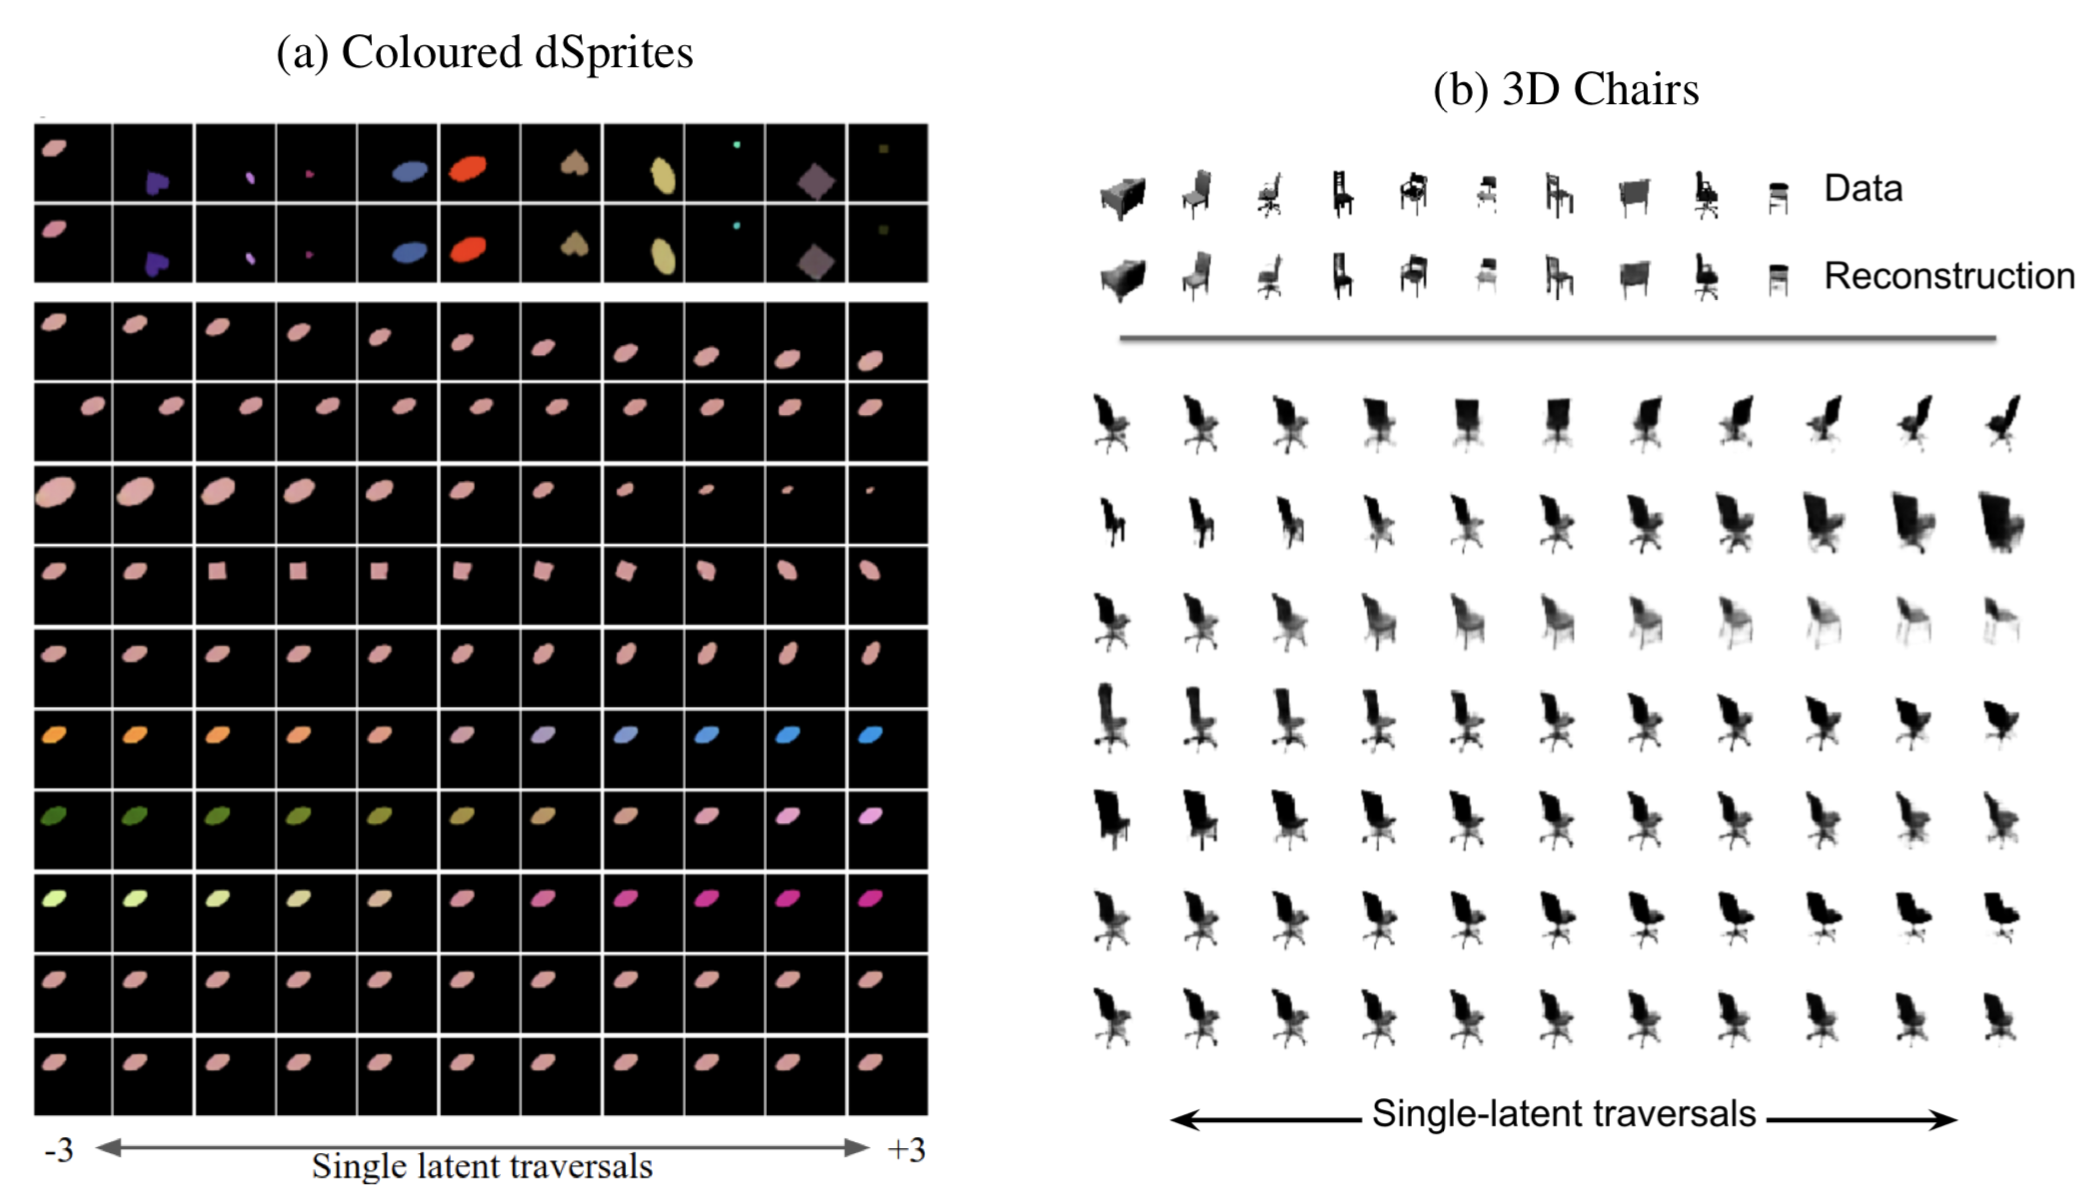
\includegraphics[width=\linewidth]{figs/betaVAE_9.png}
	\end{figure}
	\end{block}
\vfill
\hrule\medskip
{\scriptsize \href{https://arxiv.org/pdf/1804.03599.pdf}{https://arxiv.org/pdf/1804.03599.pdf}}
\end{frame}
%=======
\begin{frame}{$\beta$-VAE}
	\begin{block}{ELBO}
		\vspace{-0.3cm}
		\[
		\mathcal{L}(q, \btheta) = \frac{1}{n} \sum_{i=1}^n \left[ \mathbb{E}_{q(\bz_i | \bx_i)} \log p(\bx_i | \bz_i, \btheta) - \beta \cdot KL(q(\bz_i | \bx_i) || p(\bz_i)) \right].
		\]
		\vspace{-0.3cm}
	\end{block}
	\begin{block}{ELBO surgery}
		\vspace{-0.3cm}
		{\footnotesize
			\[
			\mathcal{L}(q, \btheta) = \underbrace{\frac{1}{n} \sum_{i=1}^n \mathbb{E}_{q(\bz_i | \bx_i)} \log p(\bx_i | \bz_i, \btheta)}_{\text{Reconstruction loss}} - \beta \cdot \underbrace{\mathbb{I}_{q(i, \bz)} [i, \bz]\vphantom{\sum_{i=1}}}_{\text{Mutual info}} - \beta \cdot \underbrace{KL(q(\bz) || p(\bz))\vphantom{\sum_{i=1}}}_{\text{Marginal KL}}
			\]}
	\end{block}
	\begin{block}{Minimization of MI}
	\begin{itemize}
		\item It is not necessary and not desirable for disentanglement. 
		\item It hurts reconstruction.
	\end{itemize}
	\end{block}
	\vfill
	\hrule\medskip
	{\scriptsize \href{https://arxiv.org/pdf/1804.03599.pdf}{https://arxiv.org/pdf/1804.03599.pdf}}
\end{frame}
%=======
\begin{frame}{DIP-VAE}
	\begin{block}{Disentangled aggregated variational posterior}
		\vspace{-0.3cm}
		\[
		q(\bz) = \bbE_{\pi(\bx)} q(\bz | \bx) = \int q(\bz | \bx) \pi(\bx) d\bx = \prod_{j=1}^d q(z_j)
		\]
		\vspace{-0.3cm}
	\end{block}
	Variational inference with disentangled prior encourages inferring factors that are close to being disentangled:
	\[
		KL(q(\bz) || \bbE_{\pi(\bx)} p(\bz | \bx)) \leq \bbE_{\pi(\bx)} KL(q(\bz | \bx) || p(\bz | \bx))	
	\]
	\begin{block}{DIP-VAE Objective}
		\vspace{-0.3cm}
		{\footnotesize
			\begin{multline*}
			\mathcal{L}(q, \btheta) = \underbrace{\bbE_{\pi(\bx)} \left[ \mathbb{E}_{q(\bz | \bx)} \log p(\bx | \bz, \btheta) - KL(q(\bz | \bx) || p(\bz)) \right]}_{\text{ELBO}} -\lambda \cdot KL(q(\bz) || p(\bz)) = \\
			= \underbrace{\bbE_{\pi(\bx)} \left[\mathbb{E}_{q(\bz | \bx)} \log p(\bx | \bz, \btheta)\right]}_{\text{Reconstruction loss}} - \underbrace{\mathbb{I}_{q(i, \bz)} [i, \bz]}_{\text{Mutual info}} - (1 + \lambda) \cdot \underbrace{KL(q(\bz) || p(\bz))}_{\text{Marginal KL}}
			\end{multline*}
		}
		\vspace{-0.3cm}
	\end{block}

	\vfill
	\hrule\medskip
	{\scriptsize \href{https://arxiv.org/abs/1711.00848}{https://arxiv.org/abs/1711.00848}}
\end{frame}
%=======
\begin{frame}{DIP-VAE}
	\begin{block}{DIP-VAE Objective}
		\vspace{-0.3cm}
		{\footnotesize
			\[
				\mathcal{L}(q, \btheta) = \underbrace{\bbE_{\pi(\bx)} \left[ \mathbb{E}_{q(\bz | \bx)} \log p(\bx | \bz, \btheta) - KL(q(\bz | \bx) || p(\bz)) \right]}_{\text{ELBO}} -\lambda \cdot KL(q(\bz) || p(\bz))
			\]
		}
		\vspace{-0.3cm}
	\end{block}
	\begin{itemize}
		\item $KL(q(\bz) || p(\bz))$ is intractable.
		\item Let match the moments of $q(\bz)$ and $p(\bz)$.
		\[
		\text{cov}_{q(\bz)}(\bz) = \bbE_{\pi(\bx)} \text{cov}_{q(\bz|\bx)}(\bz) + \text{cov}_{\pi(\bx)} \left( \bbE_{q(\bz | \bx)}\bz \right).
		\]
		For most common case $q(\bz | \bx) = \cN(\bmu(\bx), \bSigma(\bx))$:
		\[
		\text{cov}_{q(\bz)}(\bz) = \bbE_{\pi(\bx)} \bSigma(\bx) + \text{cov}_{\pi(\bx)} \bmu(\bx)
		\]
		DIP-VAE regularizes $\text{cov}_{q(\bz)}(\bz) $ to be close to the identity matrix.
	\end{itemize}
	
	\vfill
	\hrule\medskip
	{\scriptsize \href{https://arxiv.org/abs/1711.00848}{https://arxiv.org/abs/1711.00848}}
\end{frame}
%=======
\begin{frame}{DIP-VAE}
	\begin{block}{DIP-VAE Objective}
		\vspace{-0.3cm}
		{\footnotesize
			\[
			\mathcal{L}(q, \btheta) = \underbrace{\bbE_{\pi(\bx)} \left[ \mathbb{E}_{q(\bz | \bx)} \log p(\bx | \bz, \btheta) - KL(q(\bz | \bx) || p(\bz)) \right]}_{\text{ELBO}} -\lambda \cdot KL(q(\bz) || p(\bz))
			\]
		}
		\vspace{-0.5cm}
	\end{block}
	\[
		\text{cov}_{q(\bz)}(\bz) = \bbE_{\pi(\bx)} \bSigma(\bx) + \text{cov}_{\pi(\bx)} \bmu(\bx)
	\]
	\vspace{-0.3cm}
	\begin{block}{DIP-VAE-I}
		\vspace{-0.3cm}
		\[
			\max_{\btheta, \bphi} \text{ELBO}(\btheta, \bphi) - \lambda_1 \sum_{i \neq j} \left[\text{cov}_{\pi(\bx)} \bmu(\bx)\right]^2_{ij} - \lambda_2 \sum_{i} \left( \left[ \text{cov}_{\pi(\bx)} \bmu(\bx) \right]_{ii} - 1 \right)^2
		\]
		\vspace{-0.3cm}
	\end{block}
	\begin{block}{DIP-VAE-II}
		\vspace{-0.3cm}
		\[
			\max_{\btheta, \bphi} \text{ELBO}(\btheta, \bphi) - \lambda_1 \sum_{i \neq j} \left[\text{cov}_{q(\bz)} (\bz) \right]^2_{ij} - \lambda_2 \sum_{i} \left( \left[ \text{cov}_{q(\bz)} (\bz) \right]_{ii} - 1 \right)^2
		\]
		\vspace{-0.3cm}
	\end{block}
	
	\vfill
	\hrule\medskip
	{\scriptsize \href{https://arxiv.org/abs/1711.00848}{https://arxiv.org/abs/1711.00848}}
\end{frame}
%=======
\begin{frame}{DIP-VAE}
	\begin{figure}
		\centering
		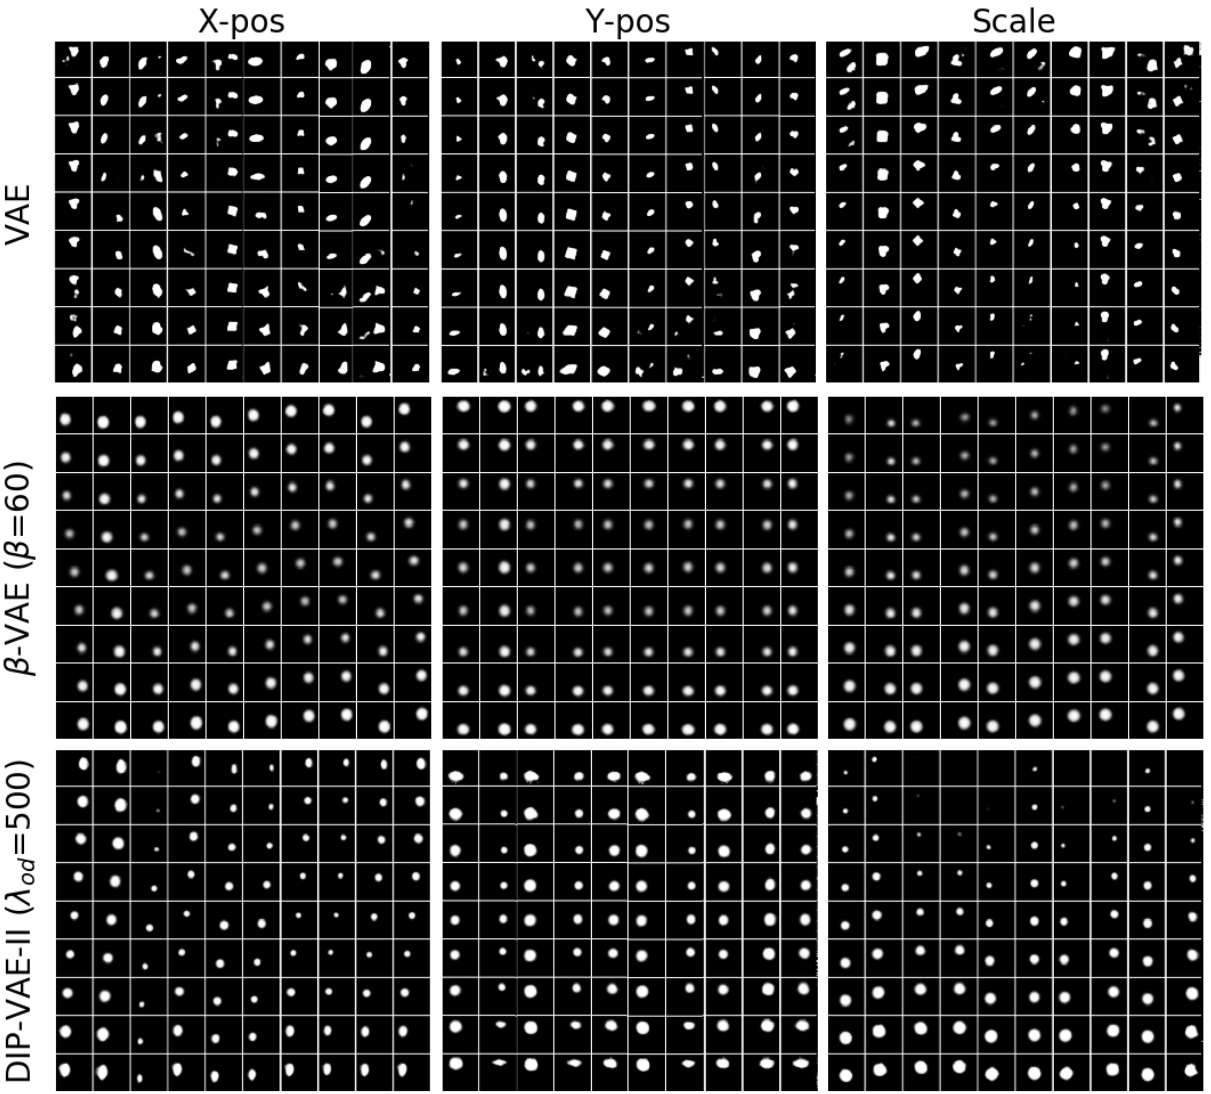
\includegraphics[width=0.8\linewidth]{figs/dip-vae_1}
	\end{figure}
	\vfill
	\hrule\medskip
	{\scriptsize \href{https://arxiv.org/abs/1711.00848}{https://arxiv.org/abs/1711.00848}}
\end{frame}
%=======
\begin{frame}{DIP-VAE}
	\begin{figure}
		\centering
		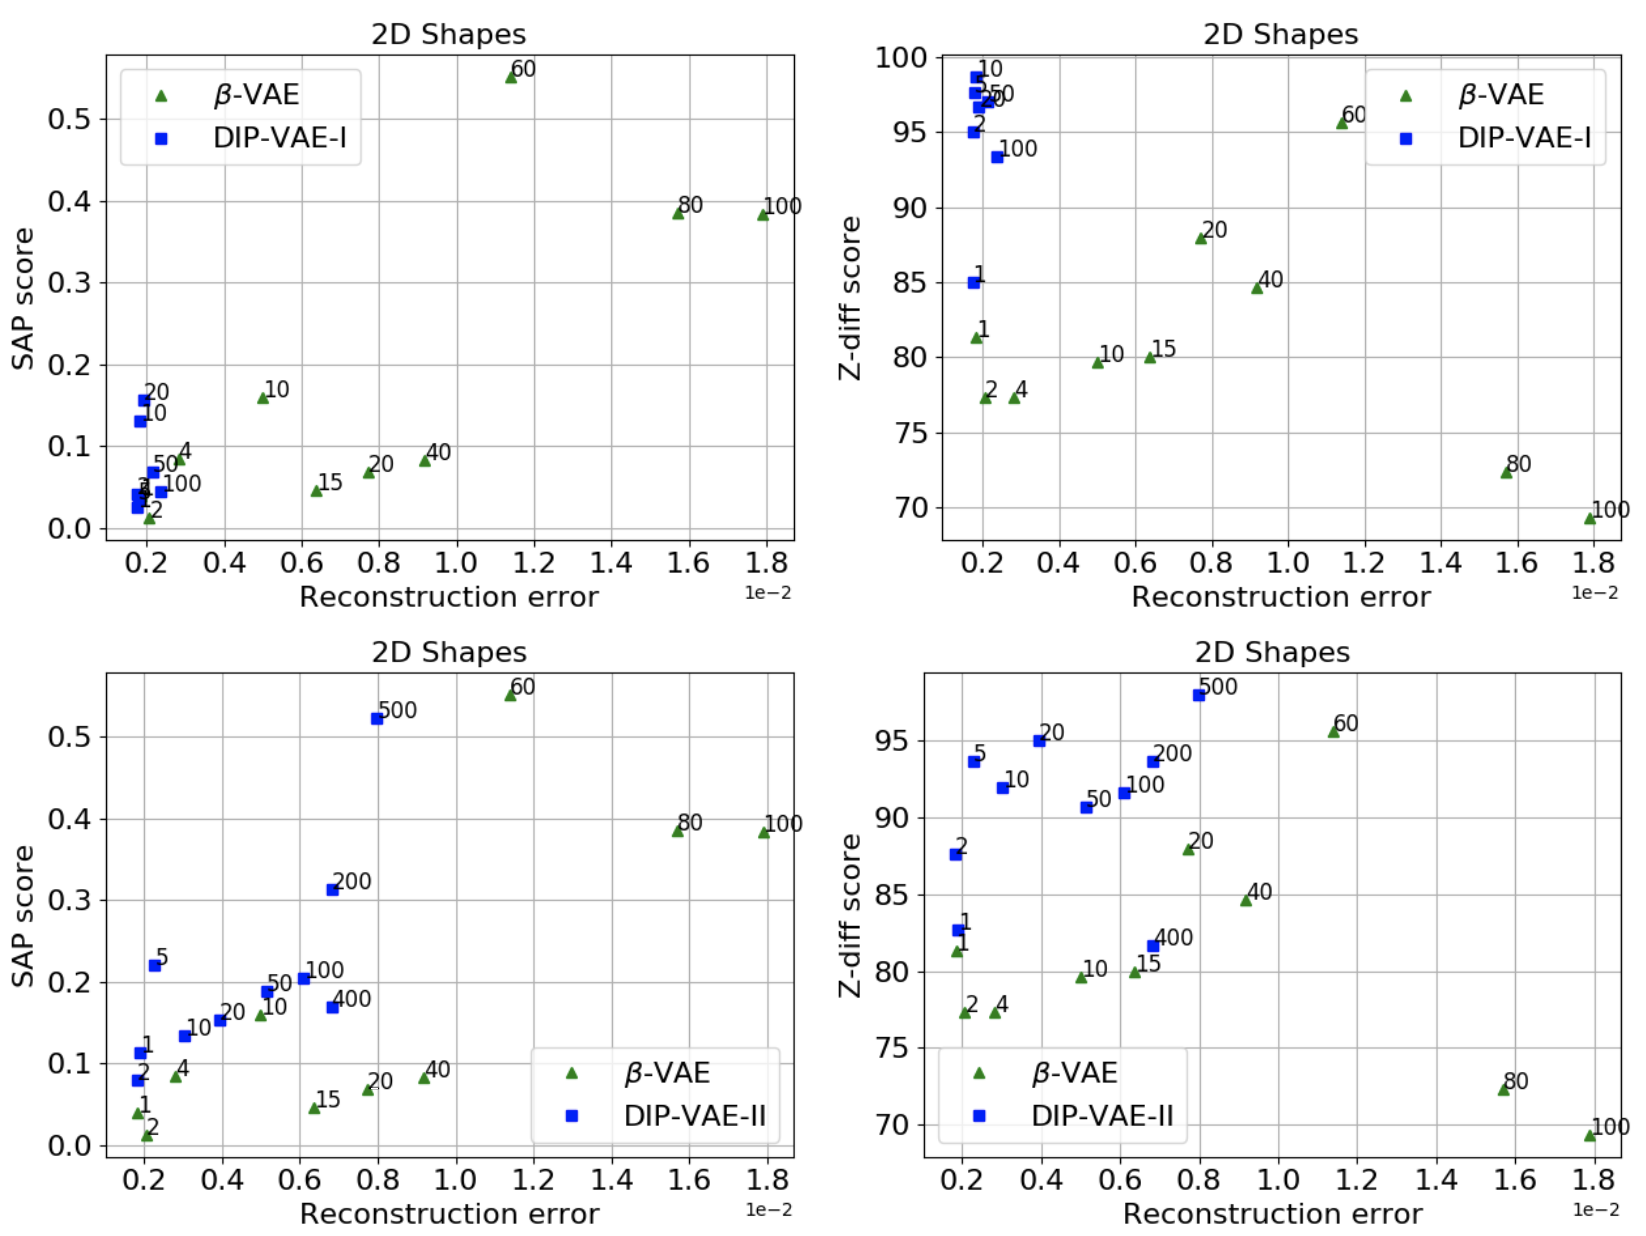
\includegraphics[width=0.95\linewidth]{figs/dip-vae_2}
	\end{figure}
	\vfill
	\hrule\medskip
	{\scriptsize \href{https://arxiv.org/abs/1711.00848}{https://arxiv.org/abs/1711.00848}}
\end{frame}
%=======
\begin{frame}{FactorVAE}
	\begin{block}{Disentangled aggregated variational posterior}
		\vspace{-0.3cm}
		\[
		q(\bz) = \bbE_{\pi(\bx)} q(\bz | \bx) = \int q(\bz | \bx) \pi(\bx) d\bx = \prod_{j=1}^d q(z_j)
		\]
		\vspace{-0.3cm}
	\end{block}
	\begin{block}{Total correlation regularizer}
		\vspace{-0.3cm}
		\[
		\min KL(q(\bz) || \prod_{j=1}^d q(z_j))
		\]
		\vspace{-0.3cm}
	\end{block}
	\begin{block}{FactorVAE objective}
		\vspace{-0.3cm}
		\[
		\min_{\btheta, \bphi} \text{ELBO}(\btheta, \bphi) - \gamma \cdot KL(q(\bz) || \prod_{j=1}^d q(z_j))
		\]
		\vspace{-0.3cm}
	\end{block}
	\begin{itemize}
		\item The last term is intractable.
		\item FactorVAE uses density ratio trick for estimation. 
	\end{itemize}
	\vspace{0.3cm}

	\vfill
	\hrule\medskip
	{\scriptsize \href{https://arxiv.org/abs/1802.05983}{https://arxiv.org/abs/1802.05983}}
\end{frame}
%=======
\begin{frame}{FactorVAE}
	Consider two distributions $q_1(\bx)$, $q_2(\bx)$ and probilistic model
	\[
		p(\bx | y) = \begin{cases}
			q_1(\bx), \text{ if } y = 1, \\
			q_2(\bx), \text{ if } y = 0,
		\end{cases}
		\quad 
		y \sim \text{Bern}(0.5).
	\]
	\begin{block}{Density ratio trick}
		\vspace{-0.5cm}
		\begin{multline*}
			\frac{q_1(\bx)}{q_2(\bx)} = \frac{p(\bx | y = 1)}{p(\bx | y = 0)} = \frac{p(y = 1 | \bx) p(\bx)}{p(y=1)} \bigg/ \frac{p(y = 0 | \bx) p(\bx)}{p(y=0)} = \\
			= \frac{p(y = 1 | \bx)}{p(y = 0 | \bx)} = \frac{p(y = 1 | \bx)}{1 - p(y = 1 | \bx)} = \frac{D(\bx)}{1 - D(\bx)}
		\end{multline*}
	Here $D(\bx)$ could be treated as a discriminator model, which outputs the probability that $\bx$ is a sample
	from $q_1(\bx)$ rather than from $q_2(\bx)$.
	\end{block}
	
	\vfill
	\hrule\medskip
	{\scriptsize \href{https://arxiv.org/abs/1802.05983}{https://arxiv.org/abs/1802.05983}}
\end{frame}
%=======
\begin{frame}{FactorVAE}
	
	\begin{block}{FactorVAE objective}
		\vspace{-0.3cm}
		\[
		\min_{\btheta, \bphi} \text{ELBO}(\btheta, \bphi) - \gamma \cdot KL(q(\bz) || \prod_{j=1}^d q(z_j))
		\]
		\vspace{-0.3cm}
	\end{block}
	
	\begin{block}{Total correlation regularizer}
		\vspace{-0.7cm}
		\begin{multline*}
		KL(q(\bz) || \prod_{j=1}^d q(z_j)) = KL(q(\bz) || \bar{q}(\bz)) = \\ =\bbE_{q(\bz)} \log \frac{q(\bz)}{\bar{q}(\bz)} \approx \bbE_{q(\bz)} \log \frac{D(\bz)}{1 - D(\bz)}
		\end{multline*}
		\vspace{-0.3cm}
	\end{block}
	VAE and GAN are trained simultaneously.
	
	\vfill
	\hrule\medskip
	{\scriptsize \href{https://arxiv.org/abs/1802.05983}{https://arxiv.org/abs/1802.05983}}
\end{frame}
%=======
\begin{frame}{FactorVAE}
	
	\begin{minipage}[t]{0.5\columnwidth}
		\begin{figure}
			\centering
			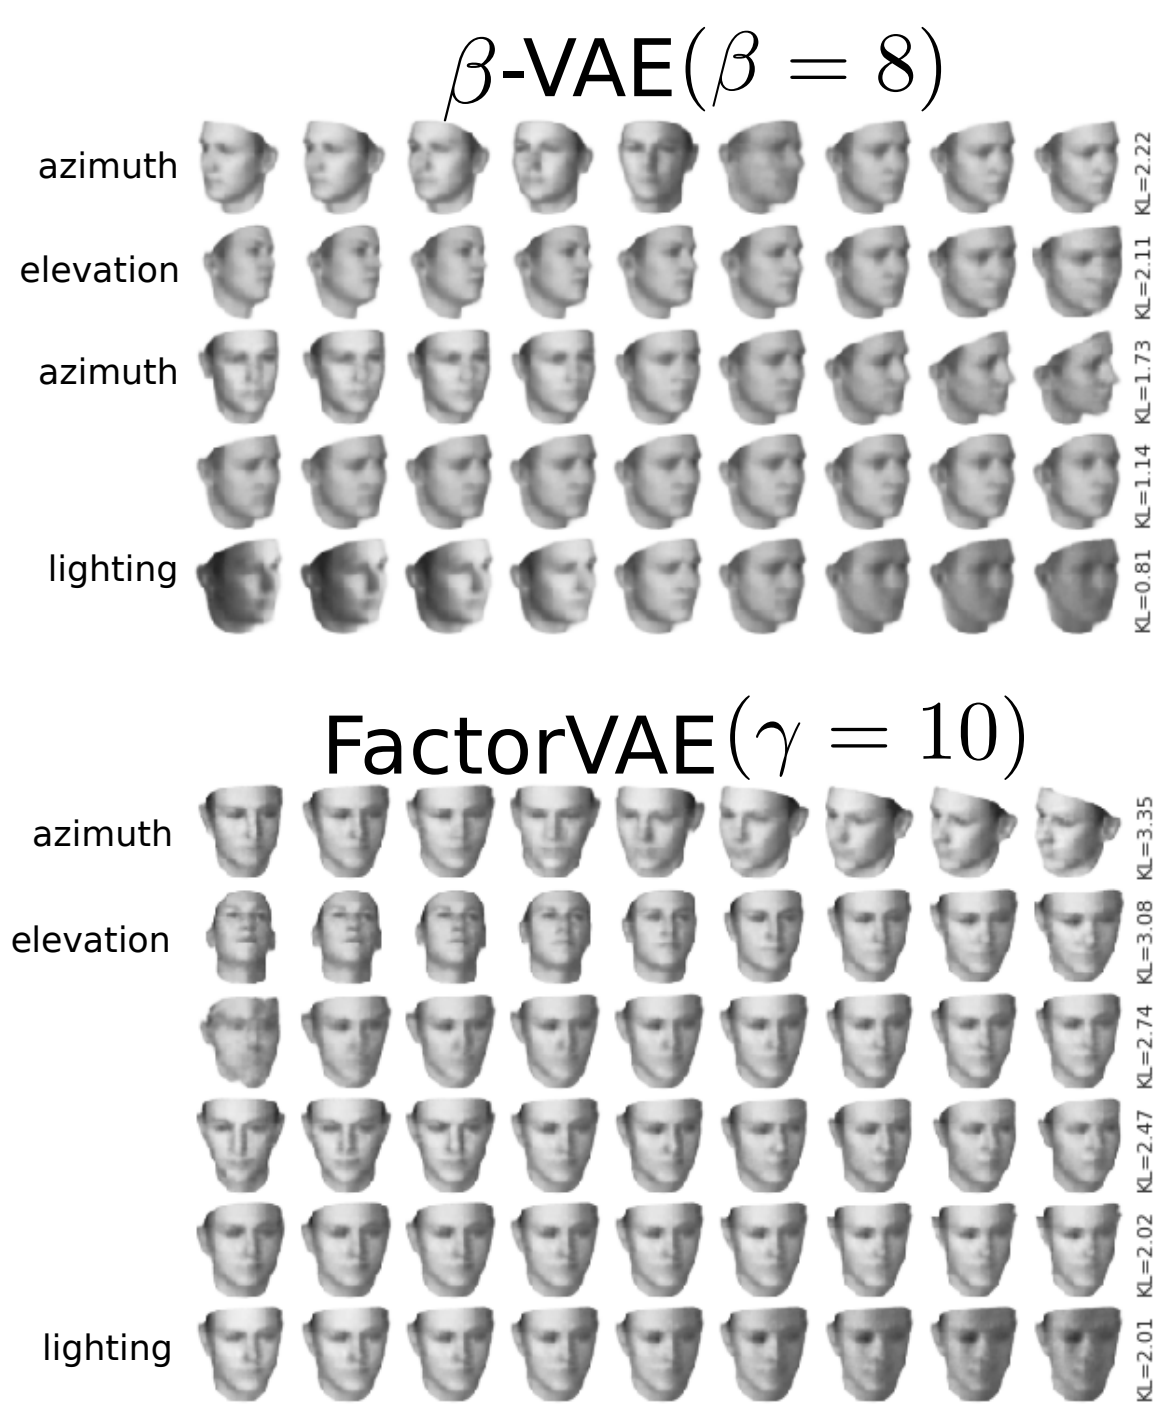
\includegraphics[width=\linewidth]{figs/factorvae_1}
		\end{figure}
	\end{minipage}%
	\begin{minipage}[t]{0.5\columnwidth}
		\vspace{1.7cm}
		\begin{figure}[h]
			\centering
			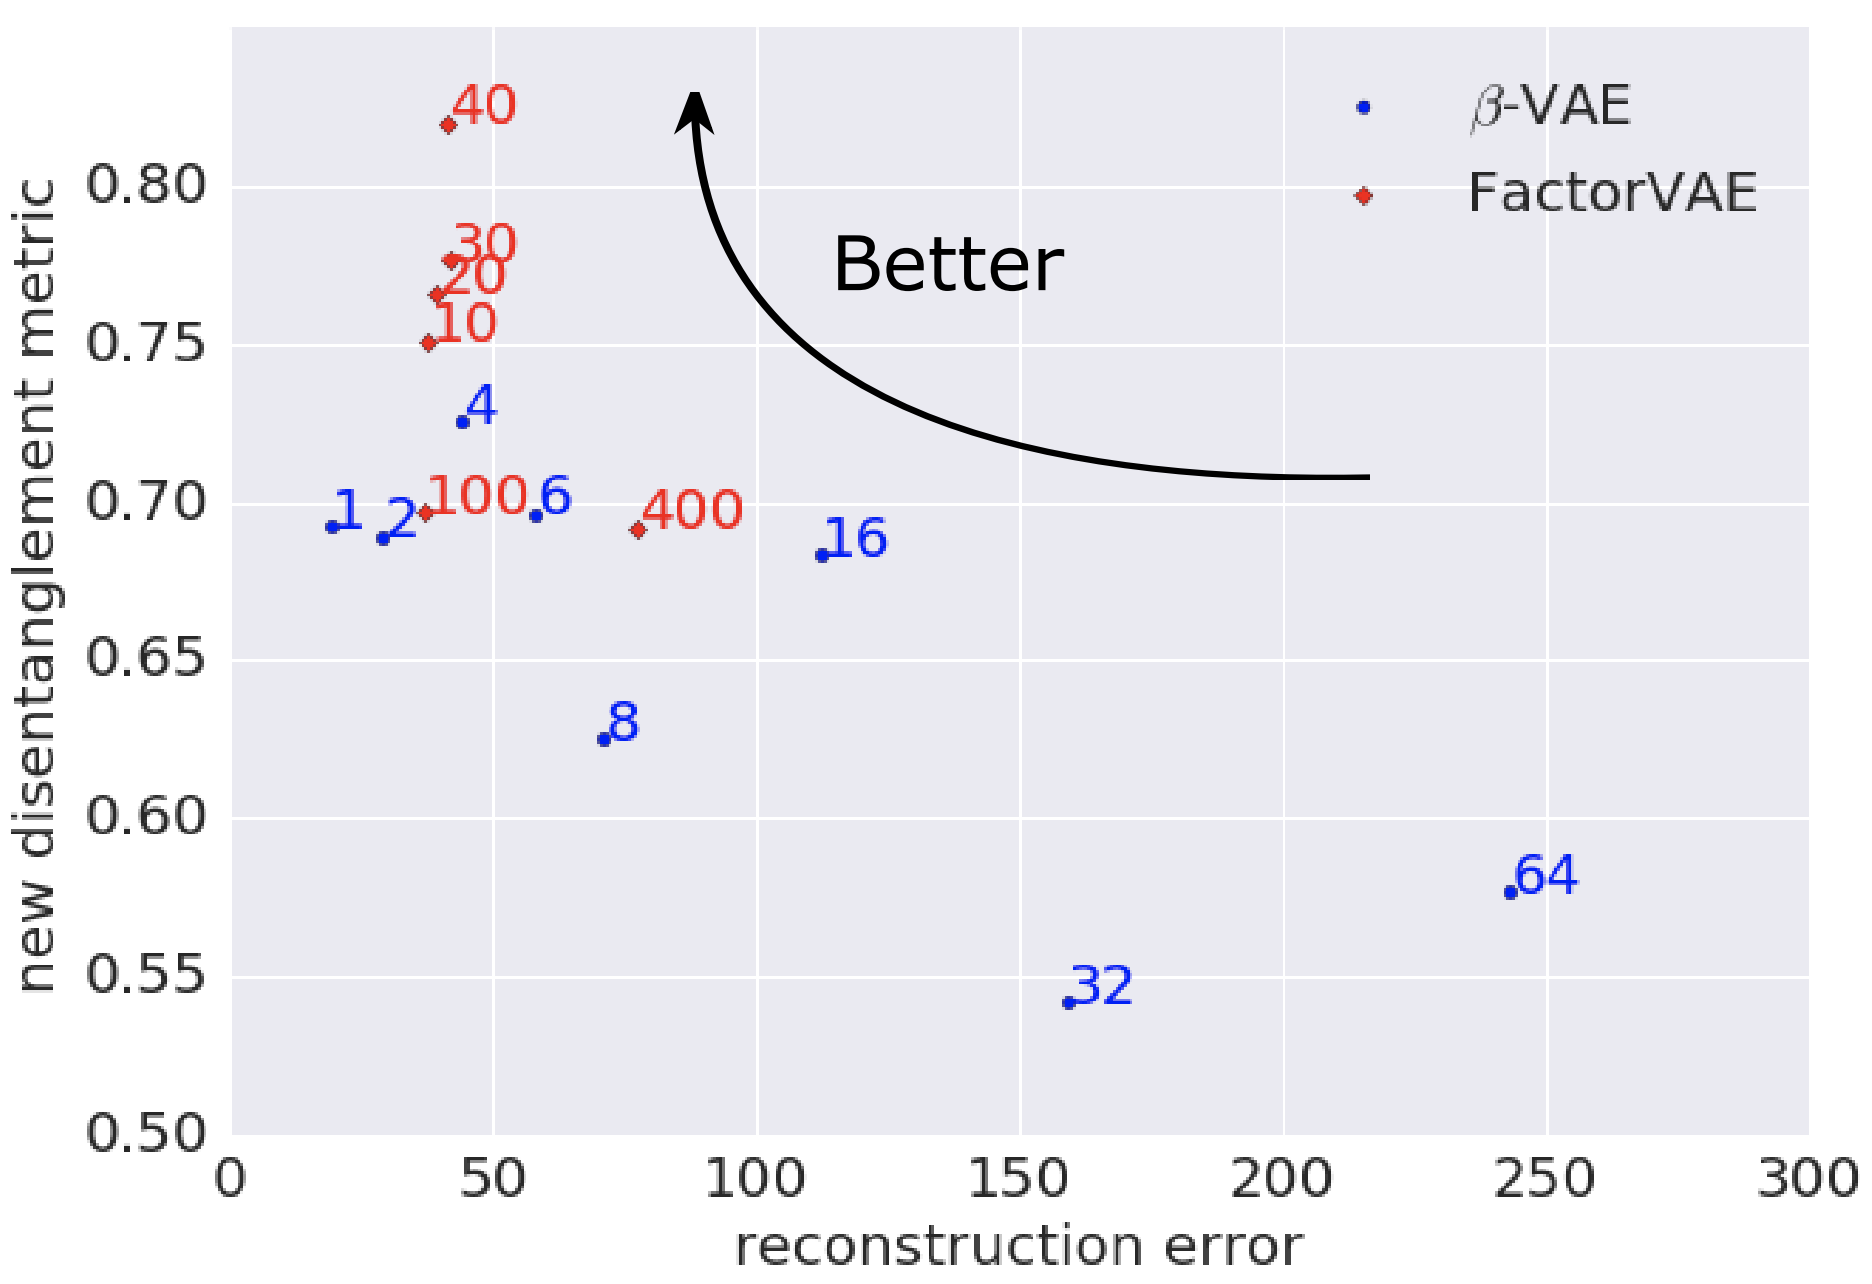
\includegraphics[width=\linewidth]{figs/factorvae_2}
		\end{figure}
	\end{minipage}
	
	\vfill
	\hrule\medskip
	{\scriptsize \href{https://arxiv.org/abs/1802.05983}{https://arxiv.org/abs/1802.05983}}
\end{frame}
%=======
\begin{frame}{Challenging Disentanglement Assumptions}
	Whether unsupervised disentanglement learning is even possible for arbitrary generative models?
	
	\begin{block}{Theorem}
		For $d > 1$, let $\bz \sim P$ denote any distribution which admits a density $p(\bz) = \prod^d_{i=1} p(z_i)$. Then, there exists an infinite family of bijective functions $f : \text{supp}(\bz) \rightarrow \text{supp}(\bz)$ such that
		\begin{itemize}
			\item $\frac{\partial f_i(\bu)}{\partial u_j} \neq 0$ almost everywhere for all $i$ and $j$ (i.e., $\bz$ and $f(\bz)$ are completely entangled);
			\item and $P(\bz \leq \bu) = P(f(\bz) \leq \bu)$ for all $\bu \in \text{supp}(\bz)$ (i.e., they
			have the same marginal distribution).
		\end{itemize}  
	\end{block}

	Theorem claims that unsupervised disentanglement learning is impossible for arbitrary generative models with a factorized prior.
	
	\vfill
	\hrule\medskip
	{\scriptsize \href{https://arxiv.org/abs/1811.12359}{https://arxiv.org/abs/1811.12359}}
\end{frame}
%=======
\begin{frame}{Challenging Disentanglement Assumptions}
	Assume we have $p(\bz)$ and some $p(\bx|\bz)$ defining a generative model. Consider any unsupervised
	disentanglement method and assume that it finds a representation that is perfectly disentangled with respect
	to $\bz$ in the generative model.
	\begin{itemize}
		\item Theorem claims that $\exists$ $\hat{\bz} = f(\bz)$ where $\hat{\bz}$ is completely entangled
		with respect to $\bz$.
		\item Since the (unsupervised) disentanglement method only has access to
		observations $\bx$, it hence cannot distinguish between the two equivalent generative models and thus has to be entangled to at least one of them
		\[
			p(\bx) = \int p(\bx | \bz) p(\bz) d\bz = \int p(\bx | \hat{\bz})p(\hat{\bz}) d \hat{\bz}.
		\]
	\end{itemize}
	
	\vfill
	\hrule\medskip
	{\scriptsize \href{https://arxiv.org/abs/1811.12359}{https://arxiv.org/abs/1811.12359}}
\end{frame}
%=======
\begin{frame}{Challenging Disentanglement Assumptions}
	\begin{block}{Proof (1)}
		\begin{enumerate}
			\item 
			Consider the function $g: \text{supp}(\bz) \rightarrow [0, 1]^d$:
			\vspace{-0.1cm}
			\[
				g_i(\bv) = P(z_i \leq v_i), \quad i=1, \dots, d.
			\]
			\vspace{-0.4cm}
			\begin{itemize}
				\item $g$ is bijective (since $p(\bz) = \prod_{i=1}dp(z_i)$).
				\item $\frac{\partial g_i(\bu)}{\partial u_i} \neq 0$, for all $i$ and $\frac{\partial g_i(\bu)}{\partial u_j} = 0$ for all $i \neq j$.
				\item $g(\bz)$ is an independent $d$-dimensional uniform distribution.
			\end{itemize}
			\item 
			Consider $h: (0, 1]^d \rightarrow \bbR^d$
			\[
				h_i(\bv) = \psi^{-1}(v_i), \quad i= 1, \dots, d.
			\]
			Here $\psi$  denotes the CDF of a standard normal distribution.
			\begin{itemize}
				\item $h$ is bijective.
				\item $\frac{\partial g_i(\bu)}{\partial u_i} \neq 0$, for all $i$ and $\frac{\partial g_i(\bu)}{\partial u_j} = 0$ for all $i \neq j$.
				\item $h(g(\bz))$  is a $d$-dimensional standard normal distribution.
			\end{itemize}
		\end{enumerate}
	\end{block}
	
	\vfill
	\hrule\medskip
	{\scriptsize \href{https://arxiv.org/abs/1811.12359}{https://arxiv.org/abs/1811.12359}}
\end{frame}
\begin{frame}{Challenging Disentanglement Assumptions}
	\begin{block}{Proof (2)}
		Let $\bA \in \bbR^{d \times d}$ be an arbitrary orthogonal matrix with $A_{ij} \neq 0$ for all $i, j$.
		The family of such matrices is infinite.
		\begin{itemize}
			\item $\bA$ is orthogonal, it is invertible and thus defines a bijective linear operator. 
			\item $\bA h(g(\bz)) \in \bbR^d$ is hence an independent, multivariate standard normal distribution.
			\item $h^{-1}( \bA h(g(\bz))) \in \bbR^d$ is an independent $d$-dimensional uniform distribution.
		\end{itemize}
		Define $f: \text{supp}(\bz) \rightarrow \text{supp}(\bz)$:
		\[
			f(\bu) = g^{-1} (h^{-1}( \bA h(g(\bz)))).
		\]
		By definition $f(\bz)$ has the same marginal distribution as $\bz$: $P(\bz \leq \bu) = P(f(\bz) \leq \bu)$ and $\frac{\partial f_i(\bu)}{\partial u_j} \neq 0$.
		\end{block}
	
	\vfill
	\hrule\medskip
	{\scriptsize \href{https://arxiv.org/abs/1811.12359}{https://arxiv.org/abs/1811.12359}}
\end{frame}
%=======
\begin{frame}{Challenging Disentanglement Assumptions}
	\begin{itemize}
		\item \textbf{Training:} Factorizing \textbf{samples} from aggregated posterior $q(\bz) = \prod_{i=1}^d q(z_i)$.
		\item \textbf{Inference:} Use the \textbf{mean} vector (usually mean of Gaussian encoder) as the representation.
	\end{itemize}
	\begin{figure}
		\centering
		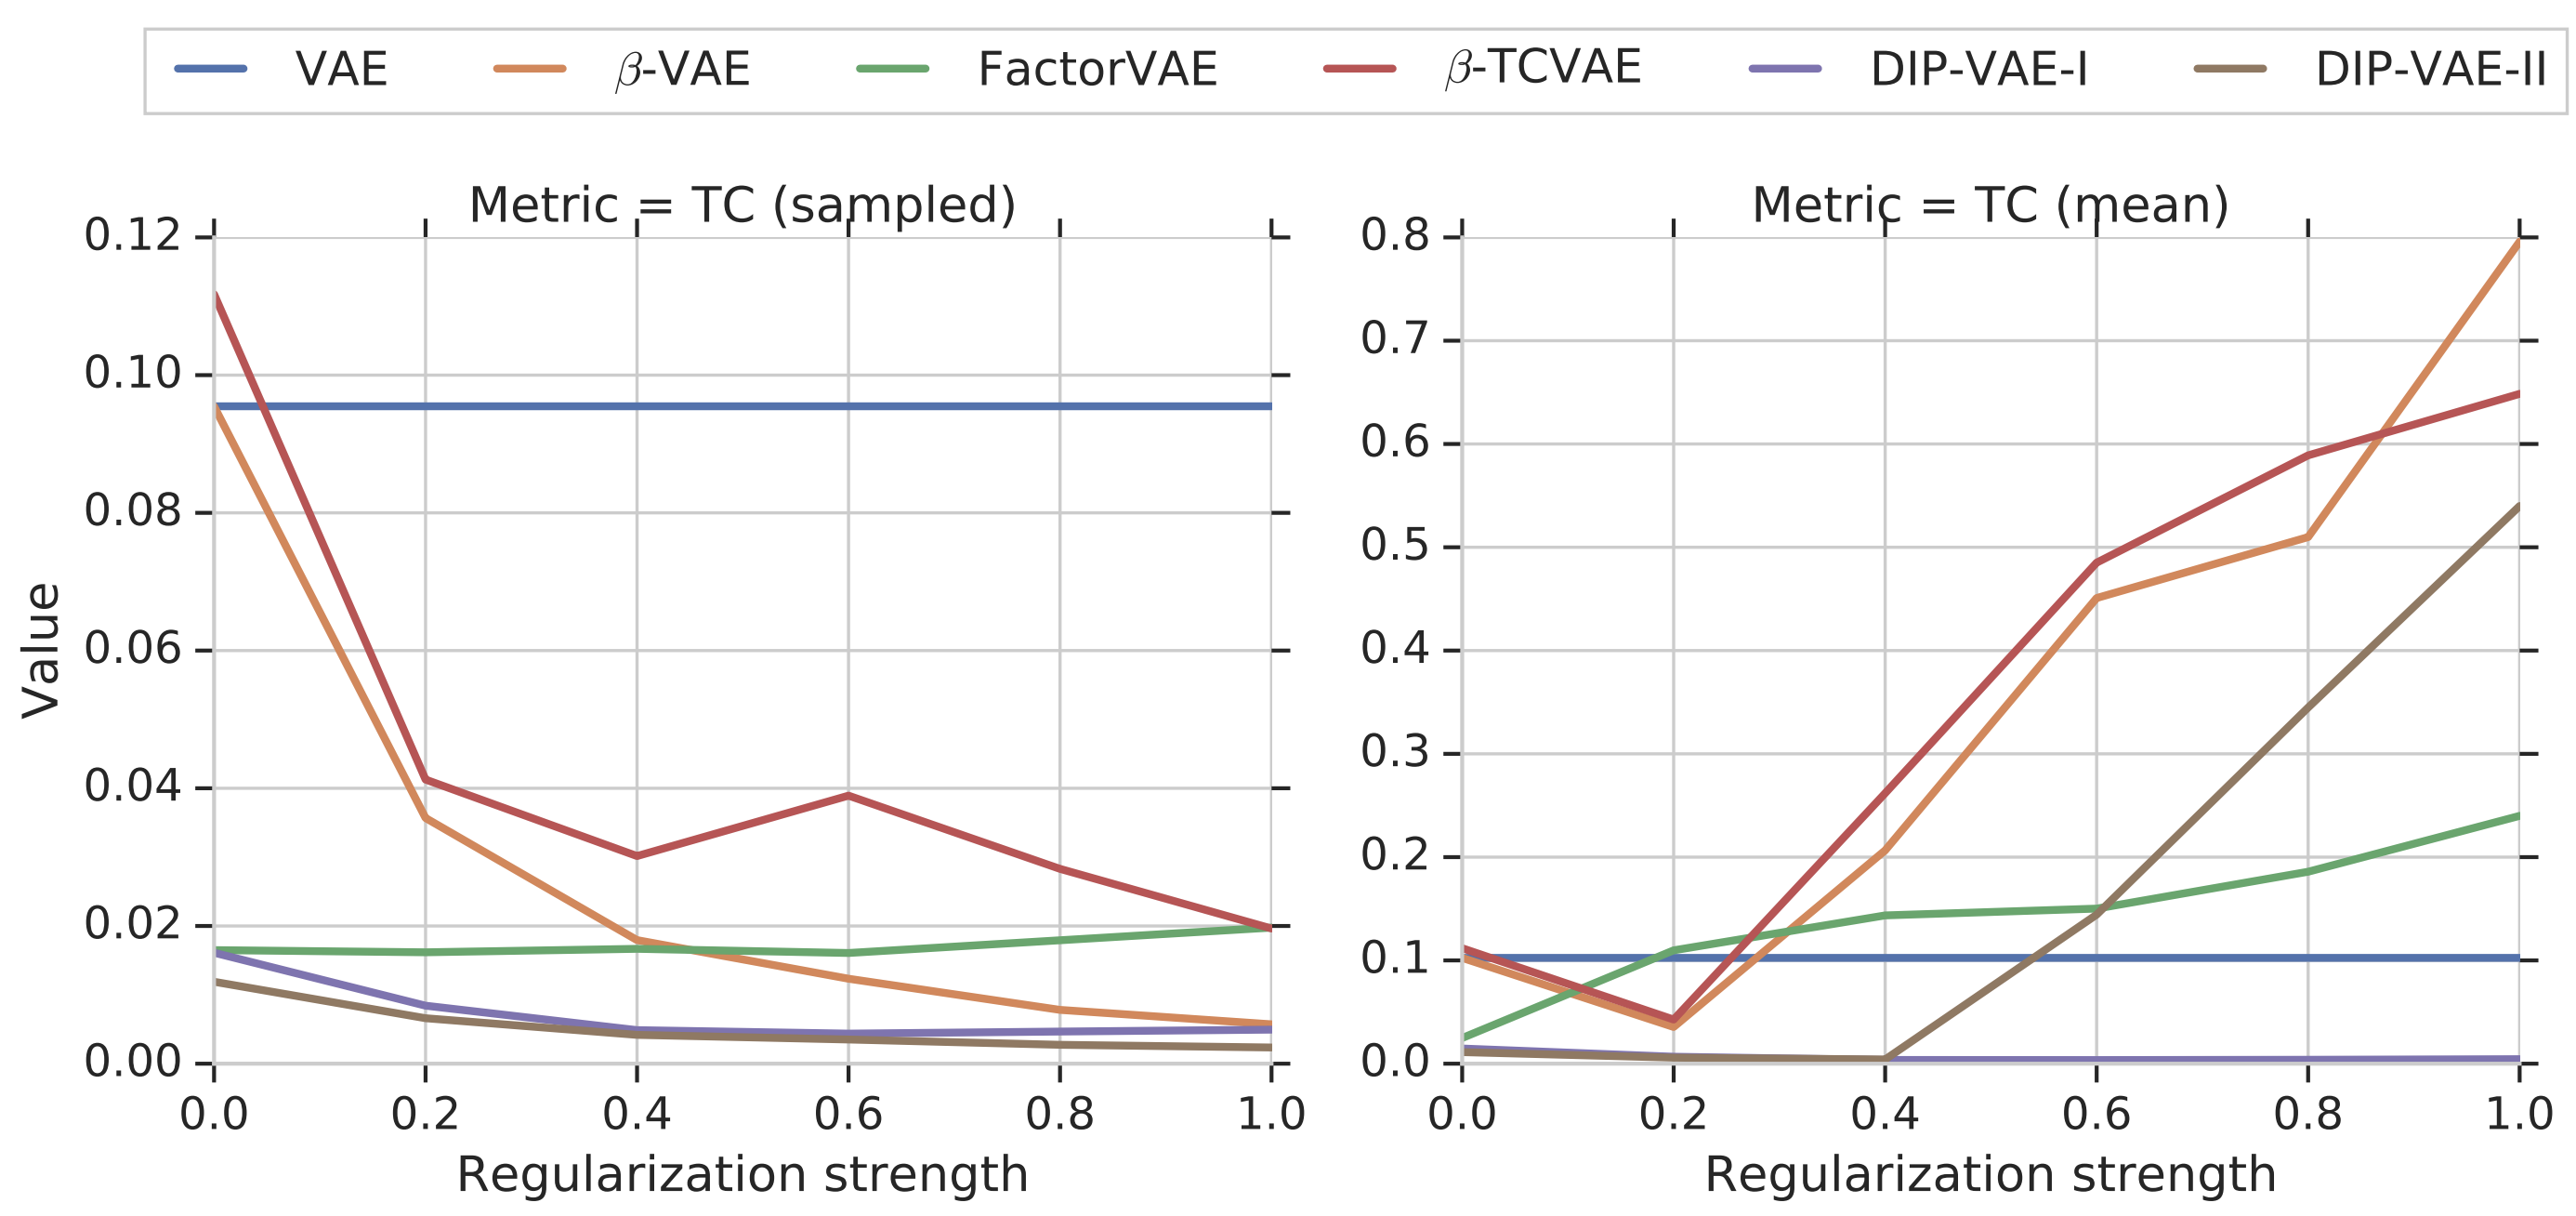
\includegraphics[width=0.95\linewidth]{figs/challenge_dis_1}
	\end{figure}
	\vfill
	\hrule\medskip
	{\scriptsize \href{https://arxiv.org/abs/1811.12359}{https://arxiv.org/abs/1811.12359}}
\end{frame}
%=======
\begin{frame}{Challenging Disentanglement Assumptions}
	\begin{block}{Importance of different models and hyperparameters for disentanglement}
		\begin{figure}
			\centering
			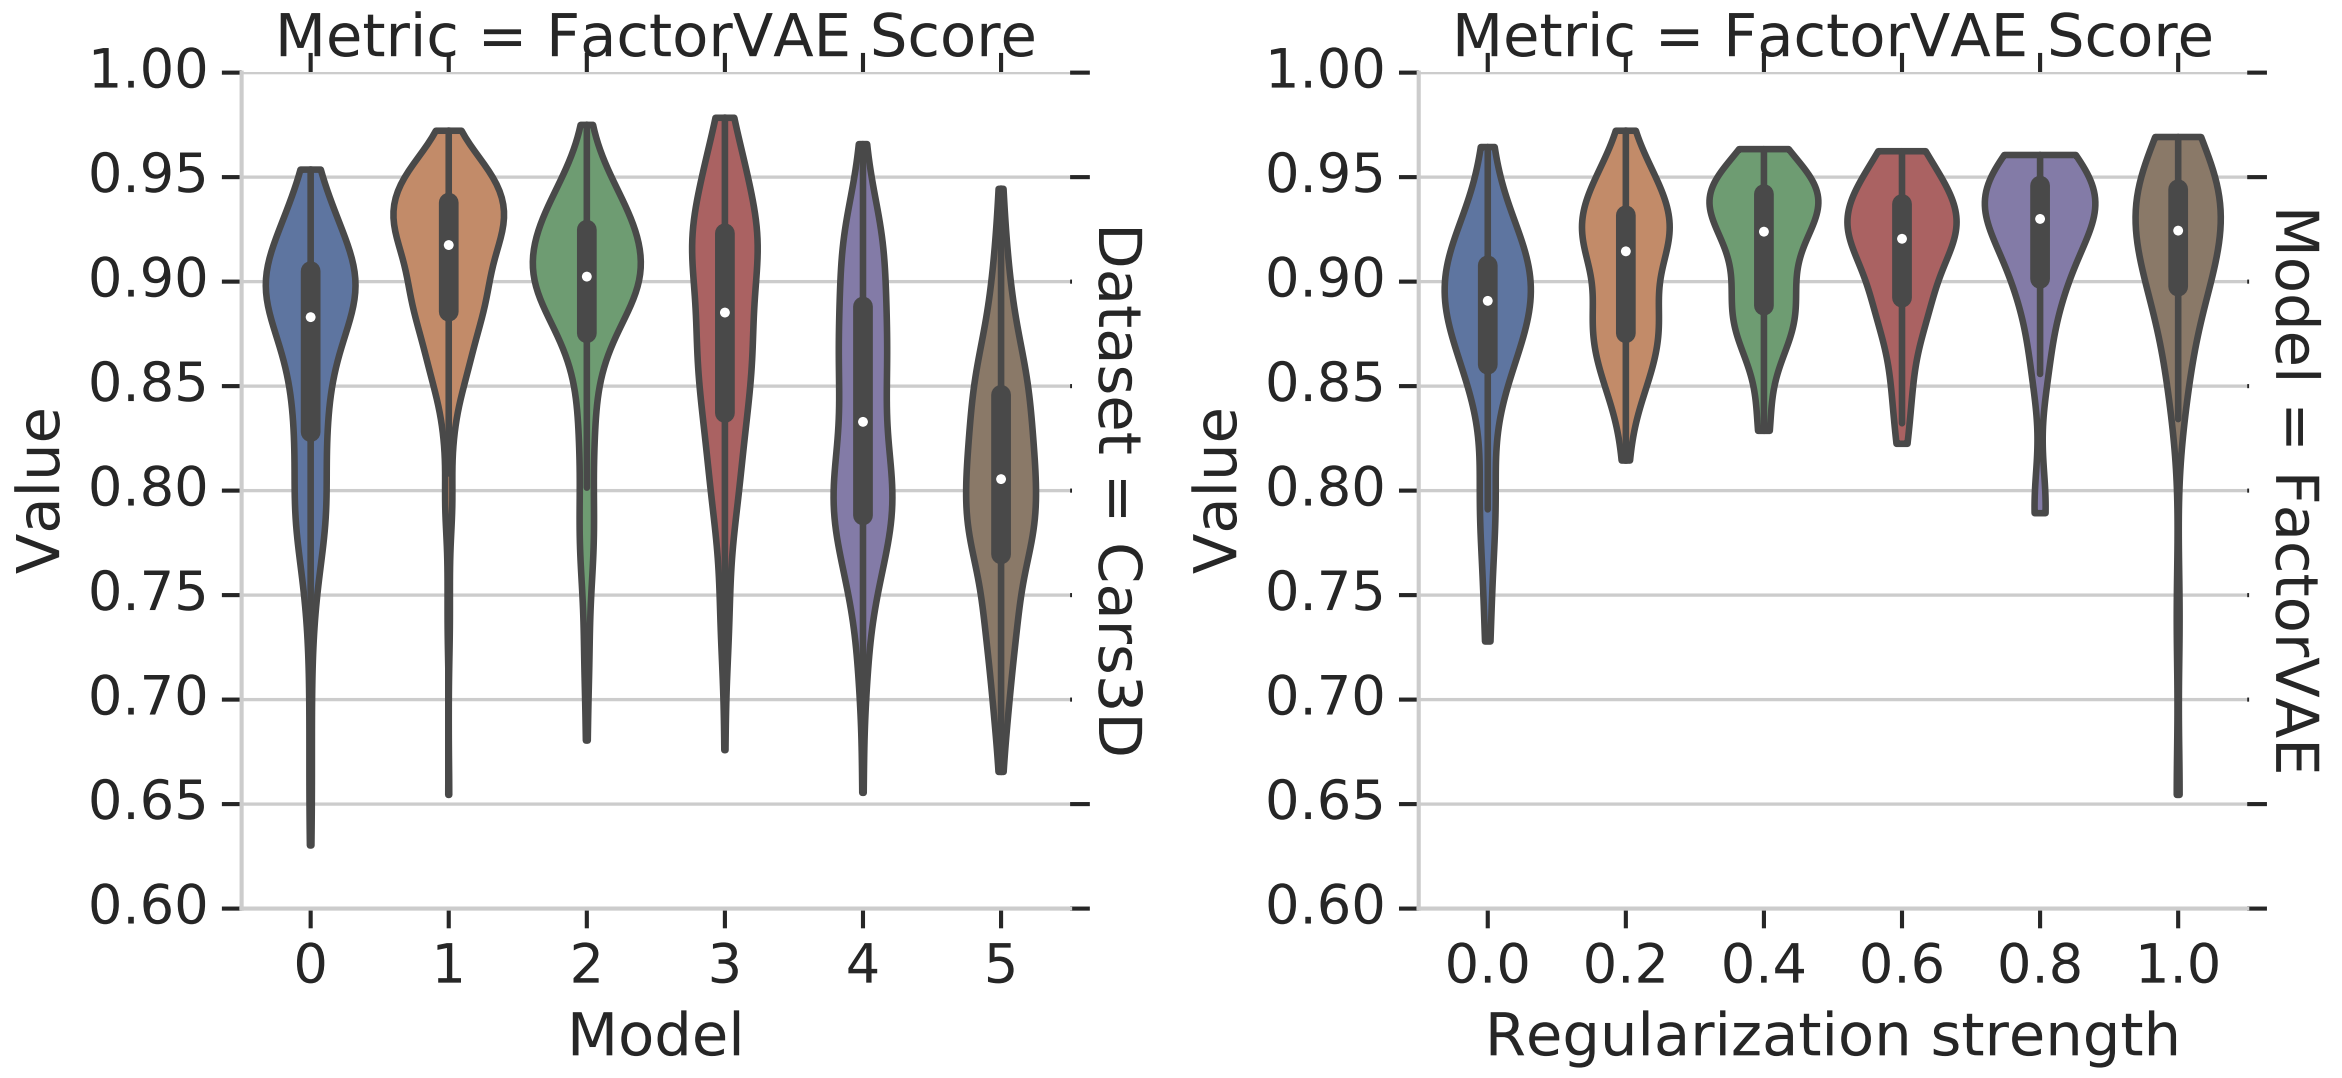
\includegraphics[width=\linewidth]{figs/challenge_dis_2}
		\end{figure}
	\end{block}
	\vfill
	\hrule\medskip
	{\scriptsize \href{https://arxiv.org/abs/1811.12359}{https://arxiv.org/abs/1811.12359}}
\end{frame}
%=======
\begin{frame}{Challenging Disentanglement Assumptions}
	\begin{block}{Agreement of different disentanglement metrics}
		\begin{figure}
			\centering
			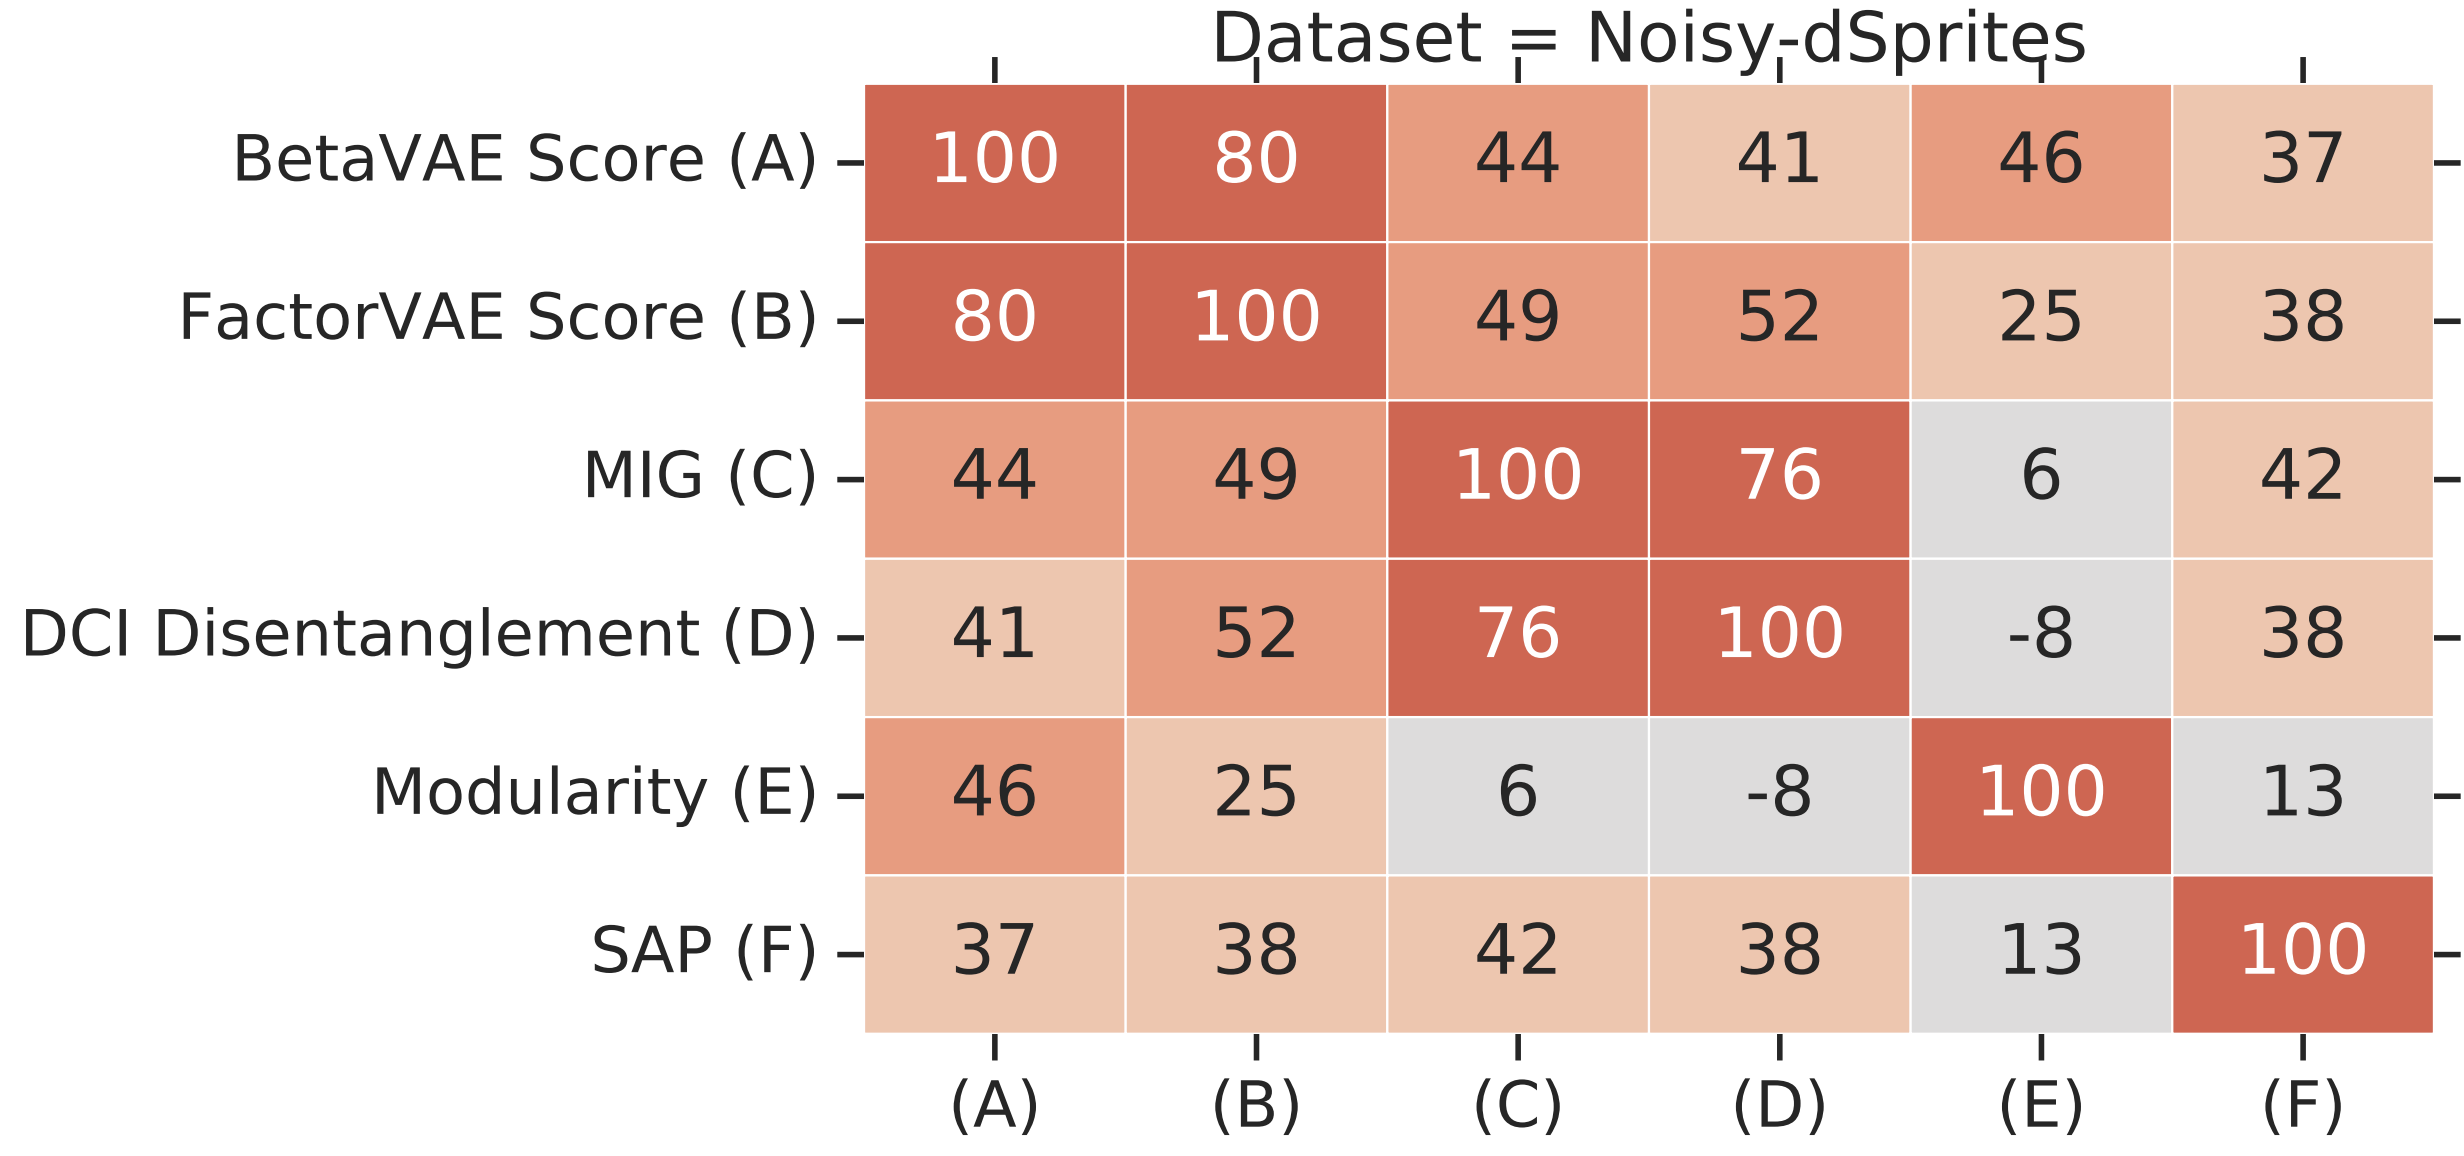
\includegraphics[width=0.9\linewidth]{figs/challenge_dis_3}
		\end{figure}
		\vspace{0.5cm}
	\end{block}
	\vfill
	\hrule\medskip
	{\scriptsize \href{https://arxiv.org/abs/1811.12359}{https://arxiv.org/abs/1811.12359}}
\end{frame}
%=======
\begin{frame}{References}
{\tiny
\begin{itemize}
	
	\item \textbf{InfoGAN:} Interpretable Representation Learning by Information Maximizing Generative Adversarial Nets \\
	\href{https://arxiv.org/abs/1606.03657}{https://arxiv.org/abs/1606.03657} \\
	\textbf{Summary:} An information-theoretic extension to the GANs that disentangles representations in an unsupervised manner. InfoGAN maximizes the MI between a small subset of the latent variables and the observation. Lower bound for \\ MI objective is derived that can be optimized efficiently. 
    
    \item \textbf{beta-VAE:} Learning Basic Visual Concepts with a Constrained Variational Framework \\
    \href{https://openreview.net/references/pdf?id=Sy2fzU9gl}{https://openreview.net/references/pdf?id=Sy2fzU9gl} \\
    \textbf{Summary:} Modifications of VAE objective. The task is represented as constrained optimization. Increasing the \\ weight of KL divergence term in ELBO allows to disentangle latent space factors and makes model more interpretable. \\ The assessment of disentanglement is provided by constructing the classifier.
    
    \item Understanding disentangling in \textbf{$\beta$-VAE} \\
    \href{https://arxiv.org/pdf/1804.03599.pdf}{https://arxiv.org/pdf/1804.03599.pdf} \\
    \textbf{Summary:} Consider beta-VAE from the position of the rate-distortion theory (information bottleneck). Propose \\ the modified ELBO with controlled latent capacity.
    
    \item \textbf{DIP-VAE:} Variational Inference of Disentangled Latent Concepts from Unlabeled Observations \\
    \href{https://arxiv.org/abs/1711.00848}{https://arxiv.org/abs/1711.00848} \\
    \textbf{Summary:} Introduce a regularizer on the expectation of the approximate posterior over observed data that encourages \\ the disentanglement. Penalize the mismatch between the aggregated posterior and a factorized prior. Comparison with beta-VAE.
    
    \item \textbf{FactorVAE:} Disentangling by Factorising \\
    \href{https://arxiv.org/abs/1802.05983}{https://arxiv.org/abs/1802.05983} \\
    \textbf{Summary:} Penalizes the total correlation with density-ratio estimation. Comparison with beta-VAE. Does not degrate \\ the reconstructions.
    
    \item \textbf{FactorVAE:} Challenging Common Assumptions in the Unsupervised Learning of Disentangled Representations  \\
    \href{https://arxiv.org/abs/1811.12359}{https://arxiv.org/abs/1811.12359} \\
    \textbf{Summary:} There infinite family of equivalent generative models with entangled factors. Uncorrelated samples vs Correlated means. Agreement of all disentanglement metrics. Hyperparameter choice is crucial.
    
\end{itemize}
}
\end{frame}
\end{document} 